\PassOptionsToPackage{table}{xcolor}
% 클래스가 선택하는 참고문헌 스타일을 로컬 정리 버전으로 연결함.
\let\brlBibliographystyle\bibliographystyle
\renewcommand{\bibliographystyle}[1]{\brlBibliographystyle{brl-mathphys-ay}}
\documentclass[pdflatex,iicol,sn-mathphys-ay]{sn-jnl}
\let\bibliographystyle\brlBibliographystyle

\usepackage{graphicx}
\usepackage{amsmath}
\usepackage{amssymb}
\usepackage{comment}
\usepackage{algpseudocode}
\usepackage[linesnumbered,ruled,vlined]{algorithm2e}
\usepackage{multirow}
\usepackage[most]{tcolorbox}
\usepackage{float}
\usepackage[normalem]{ulem}
\usepackage{xcolor}
\usepackage{subcaption}
\usepackage{stmaryrd}
\usepackage{tabularx}
\usepackage{booktabs}
\usepackage{diagbox}
\usepackage{makecell}
\usepackage{tikz}
\usepackage{array}
\usepackage{setspace}
\usepackage{pifont}

\newcommand{\cmark}{\ding{51}}
\newcommand{\xmark}{\ding{55}}
\newcommand{\omark}{\ding{108}}

\definecolor{darkblue}{rgb}{0.15,0.15,0.55}
\definecolor{lightgrey}{rgb}{0.75,0.75,0.75}
\newcommand{\qedm}{\hfill $\square$}
\DeclareUnicodeCharacter{25B3}{\ensuremath{\triangle}}
\newcommand\ny[1]{{\color{magenta}{#1}}}
\newcommand\sj[1]{{\color{violet}{#1}}}
\newcommand\sh[1]{{\color{orange}{#1}}}
\newcommand\gy[1]{{\color{purple}{#1}}}
\newcommand\cp[1]{{\color{blue}{#1}}}
\newcommand\jh[1]{{\color{green}{#1}}}

\hyphenation{op-tical net-works semi-conduc-tor}
\raggedbottom

\begin{document}

% \title[When and What to Ask External Experts during Robot Task Planning under State Uncertainty]{When and What to Ask External Experts during Robot Task Planning under State Uncertainty}

\title{When and What to Query for Proactive Feedback in Robot Task Planning under Partial Observability}

\author[1]{\fnm{Changmin} \sur{Park}}\email{cmp9877@gmail.com}
\equalcont{These authors contributed equally to this work.}

\author[1]{\fnm{Seongah} \sur{Park}}\email{ppseongah@gmail.com}
\equalcont{These authors contributed equally to this work.}

\author[1]{\fnm{Nayoung} \sur{Kim}}\email{nayoungkim0826@gmail.com}
\author[1]{\fnm{Sungjin} \sur{Park}}\email{sungjin.park@sogang.ac.kr}
\author[1]{\fnm{Gayoung} \sur{Ryu}}\email{gyryu.sg@gmail.com}
\author[1]{\fnm{Geonyeong} \sur{Ko}}\email{2567bear@naver.com}
\author*[1]{\fnm{Junho} \sur{Lee}}\email{kjcom5322@gmail.com}
\author*[1,2]{\fnm{Changjoo} \sur{Nam}}\email{cjnam@sogang.ac.kr}

\affil*[1]{\orgname{Sogang University},
  \orgaddress{\city{Seoul}, \country{Republic of Korea}}}
\affil[2]{\orgname{Institution2},
  \orgaddress{\city{Seoul}, \country{Republic of Korea}}}

% \abstract{In this paper, we present a method for deciding when a robot should request external information and what it should ask during task planning. A robot operating with incomplete information may fail to determine the current state of the world, which can lead to task failure. However, resolving every such ambiguity through external queries would incur unnecessary costs. Therefore, a robot must determine both when to query and what information to request. To solve this problem, we maintain a weighted belief over possible task states. We use belief uncertainty to decide when to query and select the \cp{query content} with the highest expected uncertainty reduction to determine what to ask. After receiving an answer from an external \cp{feedback source}, the belief is updated and task execution continues. We evaluate the framework in two robotic task domains and compare it with alternative strategies for query timing and query selection. \cp{The results show that deciding when to query has a substantial effect on task success, whereas deciding what to query mainly affects the number of required queries.} Compared with \cp{conformal-prediction-based and reward-based strategies}, our method achieves higher task success, highlighting the importance of query timing and selection beyond simply minimizing the number of queries.}

\abstract{In this paper, we present a method for deciding when a robot should request external information and what it should ask during task planning. A robot operating with incomplete information may fail to determine the current state of the world, which can lead to task failure. However, resolving every such ambiguity through external queries would incur unnecessary costs. Therefore, a robot must determine both when to query and what information to request. To solve this problem, we maintain a weighted belief over possible task states. We use belief uncertainty to decide when to query and select \cp{the question about the current state expected to reduce uncertainty the most}. After receiving an answer from an external \cp{feedback source}, the belief is updated and task execution continues. \cp{We evaluate the framework on two robotic tasks against other systems that request external feedback during task planning. In simulation with correct responses, our method achieves higher success rates than the best-performing baseline across the two domains, with $100.0\%$ versus $87.00\%$ and $98.00\%$ versus $57.50\%$. The success advantage also holds with vision-language model and human feedback in real-world experiments.}}



\keywords{Planning under uncertainty, online symbolic planning, robotic systems}

\maketitle

\section{Introduction}~\label{intro}
% Robots operating in real-world environments often have incomplete or unreliable information about the current state due to perception errors~\citep{kaipa2016addressing}, execution failures~\citep{kaelbling1998planning}, and unexpected environmental changes~\citep{kurniawati2016online}. If such uncertainty is not resolved, the robot may make incorrect decisions and fail the task. \cp{The robot can proactively request information from an external feedback source to reduce this uncertainty~\citep{dragan2013legibility, goodrich2008human}. However, frequent queries can incur substantial costs in time and workload~\citep{chen2014human}.} The robot must therefore determine \textit{when} external information is necessary and \textit{what} information should be requested.
Robots operating in real-world environments often have incomplete or unreliable information about the current state due to perception errors~\citep{kaipa2016addressing}, execution failures~\citep{kaelbling1998planning}, and unexpected environmental changes~\citep{kurniawati2016online}. If such uncertainty is not resolved, the robot may make incorrect decisions and fail the task. In practice, relying on an external agent to recognize the need for assistance requires continuous monitoring of robot execution. The robot must therefore be able to detect uncertainty and initiate queries to obtain additional information before proceeding~\citep{dragan2013legibility, goodrich2008human}. However, frequent queries can incur substantial costs in time and workload~\citep{chen2014human}. The robot must therefore determine \textit{when} to request external feedback and \textit{what} to ask from the available query candidates.
% Robots operating in real-world environments often have incomplete or unreliable information about the current task state due to perception errors~\cite{kaipa2016addressing}, execution failures~\cite{kaelbling1998planning}, and unexpected environmental changes~\cite{kurniawati2016online}. If such uncertainty is not resolved, the robot may make incorrect decisions and fail the task. External information from an expert can help resolve this uncertainty~\cite{dragan2013legibility, goodrich2008human}, but frequent queries can incur substantial costs in time and workload~\cite{chen2014human}. The robot must therefore determine \textit{when} external information is necessary and \textit{what} information should be requested.

% Recent uncertainty-aware systems selectively request external feedback during task execution. Existing approaches commonly trigger queries based on prediction confidence, including conformal prediction~\citep{ren2023robots, liang2024introspective, mullen2025lbap}, or on the expected effect of a query on task reward~\citep{burks2021collaborative, anand2025adaptive}. \cp{However, a confident action prediction does not ensure that the underlying state estimate is correct. Under reward-based criteria, the robot may also execute an action without querying even when state uncertainty remains. Both approaches can therefore miss opportunities to verify the state information needed for successful execution, leading to task failure. We use state uncertainty to determine when verification is needed and expected uncertainty reduction to select what to ask.}
Existing proactive querying methods often use action prediction confidence or expected return to guide querying decisions. For example, KnowNo uses conformal prediction sets to determine when to request an action choice~\citep{ren2023robots}, while IntroPlan combines conformal prediction with retrieved reasoning examples for candidate evaluation~\citep{liang2024introspective}. Yet both methods may proceed without querying if incorrect perception produces a confident action prediction. Even when assistance is requested, the candidate set may not include a correct action. POMDP-based approaches~\citep{burks2021collaborative,burks2023harps} model candidate queries as planning actions and determine when and what to query by maximizing expected cumulative reward. However, optimizing rewards for task performance does not necessarily yield efficient querying, because asking fewer questions can increase the risk of failure, while asking more does not always improve task success.

In this paper, we present a belief-based method for deciding when to request external feedback and what to ask. We formulate task planning as a POMDP~\citep{kaelbling1998planning} and maintain a knowledge base containing symbolic facts and STRIPS-style action models~\citep{davis1993knowledge,fikes1971strips}. After each action, the robot uses these facts and action models to generate reachable states and constructs a weighted belief using the resulting observation. If belief confidence falls below a threshold, the robot asks an external agent to verify the state fact with the greatest expected entropy reduction. The robot updates the belief after each response and continues querying until the confidence reaches the threshold. The robot then updates the facts in the knowledge base and resumes planning and execution.
% In this paper, we present a method that \cp{maintains and updates} a weighted belief over possible task states throughout execution. We formulate decision making as a partially observable Markov decision process (POMDP)~\citep{kaelbling1998planning} and represent task knowledge using a STRIPS-style symbolic model~\citep{davis1993knowledge,fikes1971strips}. The belief is updated after each action and observation, and its uncertainty is used to determine when external information is needed. If a query is triggered, the robot selects the state fact expected to reduce uncertainty the most and asks an external agent to verify it. The response is incorporated into the belief, which is then used for subsequent planning and execution.




We evaluate the method in two robotic domains. \cp{In simulation with correct oracle responses}, we compare our method with conformal-prediction-based and reward-based strategies and analyze the effects of query timing and query selection. We then conduct physical robot experiments with feedback from a vision-language model (VLM) and human participants, comparing our method with the conformal-prediction-based method. Interviews with the five participants provide qualitative insights into their experiences with both methods. Our method achieves higher task success rates than all evaluated baselines in simulation and than the selected baseline with VLM and human feedback on physical robots. Ablation results indicate that query timing primarily affects task success, while query selection reduces the number of queries required.

The contributions of this work are as follows:
\begin{itemize}
\item We determine when to query based on uncertainty in the current belief and show that query timing has a substantial effect on task success.
\item We choose what to query using expected entropy reduction and show that query selection reduces query counts compared to the baselines.
\item We evaluate the proposed method in simulation and on physical robots with VLM and human feedback, demonstrating higher task success than the evaluated baselines.
\end{itemize}

\section{Related Work}~\label{related}

\subsection{Planning under Uncertainty}~\label{rel:state_uncertainty}

Symbolic task representations such as STRIPS and PDDL~\cite{fikes1971strips,aeronautiques1998pddl} describe task-relevant objects, predicates, goals, and action transitions in an explicit form. In symbolic task planning, action applicability depends on the facts that hold in the current state~\cite{fikes1971strips,helmert2009concise}. Uncertainty about these facts can therefore affect which actions and plans are considered feasible. However, standard symbolic planning generally assumes a single current state and does not directly account for noisy observations, hidden information, or multiple competing interpretations of the world.

POMDPs provide a general framework for planning under such uncertainty by maintaining a belief over possible states and accounting for future observations when selecting actions~\cite{kaelbling1998planning,pineau2003point,ross2008online,somani2013despot}. Exact belief-space planning is often intractable, so approximate methods use structure or samples to represent the belief. Factored POMDP approaches exploit structure in state, observation, or value-function components~\cite{hansen2000dynamic,feng2001approximate,veiga2014point}. Related inference methods maintain factorized distributions for structured dynamic Bayesian networks~\cite{murphy2013factored}. These methods improve scalability but can require assumptions or approximations about dependencies among state variables.

Particle-based approaches instead approximate a belief with samples of complete states. Each particle retains a complete state hypothesis without an explicit factorization of the state distribution. Particle representations have been used for navigation and exploration~\cite{lauri2016exploration,kim2021plgrim}, object search~\cite{xiao2019objectsearch}, and manipulation~\cite{pajarinen2017multiobject,pajarinen2022composition}. Their computational cost can increase with the number of particles required to represent a large state space. In symbolic tasks, unconstrained sampling can also produce state hypotheses that are inconsistent with task dynamics. We therefore use reachable task-state particles to retain complete state hypotheses while excluding states that cannot arise under the task model.

Several works combine symbolic task knowledge with probabilistic planning. CORPP~\cite{zhang2015corpp}, for example, constructs priors over possible worlds from commonsense knowledge and incorporates them into POMDP planning. Other approaches integrate structured task representations with belief-space decision making~\cite{sanner2010symbolic,serrano2021knowledge,li2026uncertainty}. These works show how symbolic structure can organize probabilistic reasoning over task states. Building on this connection, we use a symbolic task model both to define the states in the belief and to identify the state facts available for external verification.


\subsection{Selective Querying under Uncertainty}~\label{rel:selective_querying}


System-initiated querying allows a robot to request task-relevant information from an external source when onboard observations are insufficient~\cite{ren2023robots}. This mechanism differs from active sensing, active perception, and exploration~\cite{lauri2016exploration,kim2021plgrim}. Those methods reduce uncertainty through observations generated during interaction with the environment. External querying can provide state information that onboard observations do not reveal reliably, but each query adds interaction time and workload~\cite{chen2014human}. A selective querying method must therefore determine both when external information is necessary and what information should be requested.


Prior work determines when to query using policy confidence or learned uncertainty~\cite{singi2023hula,igbinedion2024learning,mullen2025lbap}, trust in human input~\cite{mangalindan2025seek}, calibrated prediction sets~\cite{ren2023robots,liang2024introspective,zhao2025conformalized}, or the expected utility of a query~\cite{burks2021collaborative,anand2025adaptive}. KnowNo, for example, requests help when a conformal prediction set contains more than one candidate action~\cite{ren2023robots}. These criteria identify a difficult decision, estimate the value of assistance, or account for the reliability of an information source. However, ambiguity among predicted actions does not show whether missing information about the current task state caused the difficulty. We therefore determine when to query from uncertainty in an explicit belief over current task states.


The decision of what to ask is closely coupled with the decision of when to ask because the uncertainty that triggers a query also determines which information is needed. KnowNo first constructs a conformal prediction set of candidate actions and asks the user to select among them when the set contains multiple actions~\cite{ren2023robots}. Related approaches likewise request guidance over candidate actions or plans when predictions are uncertain~\cite{liang2024introspective,mullen2025lbap}. In these methods, the candidate set determines the query target before the external response is obtained. This design can resolve uncertainty about the next action when the correct action is among the candidates, but it does not necessarily resolve uncertainty about the current task state. We therefore select a planning-relevant state fact from the current belief according to its expected reduction of uncertainty.


Prior work has treated planning under state uncertainty and selective querying as separate problems. Planning methods use state uncertainty to select robot actions, whereas selective querying methods typically use decision confidence or expected utility to request assistance. Our work occupies the intersection of these directions by grounding planning, query timing, and query selection in uncertainty about the current task state.

\section{Preliminaries}~\label{preliminaries}

% The objective of planning is to find a transition sequence that transforms the initial state into a goal state. 
The planning problem is defined as a tuple $\mathcal{P} = \langle \mathcal{F}, \mathcal{A}, s_0, \mathcal{G} \rangle$, where $\mathcal{F}$ is a finite set of atoms, $\mathcal{A}$ is a set of actions, $s_0 \subseteq \mathcal{F}$ is the initial state, and $\mathcal{G} \subseteq \mathcal{F}$ is the goal condition. A state $s$ is represented as a subset of $\mathcal{F}$. Each action $a \in \mathcal{A}$ is defined as a tuple $a = \langle \mathrm{pre}(a), \mathrm{add}(a), \mathrm{del}(a) \rangle$, where $\mathrm{pre}(a), \mathrm{add}(a), \mathrm{del}(a) \subseteq \mathcal{F}$ denote the preconditions, add lists, and delete lists of the action, respectively. 
% We can say that $a$ is applicable in $s$ if and only if $\mathrm{pre}(a) \subseteq s$, denoted as $a \llbracket s \rrbracket$. 
An action $a$ is said to be applicable in state $s$ if and only if $\mathrm{pre}(a) \subseteq s$, denoted as $a \llbracket s \rrbracket$.
The state transition is defined as $s \xrightarrow{a} s^\prime$, where $s^\prime = (s \setminus \mathrm{del}(a)) \cup \mathrm{add}(a).$

A plan is a sequence of actions $\pi = (a_1, \dots, a_T)$ such that the goal condition is satisfied after sequentially applying the actions starting from the initial state, i.e.,
\[
s_0 \xrightarrow{a_1} s_1 \xrightarrow{a_2} \cdots \xrightarrow{a_T} s_T
\quad \text{and} \quad \mathcal{G} \subseteq s_T.
\]


A POMDP is defined as a tuple $\langle \mathcal{S}, \mathcal{A}, T, R, \Omega, O, \gamma \rangle$, where $\mathcal{S}$ is the state space, $\mathcal{A}$ is the action space, and $\Omega$ is the observation space. The transition model $T(s^\prime \mid s, a)$ specifies the probability of reaching the next state $s^\prime$ after taking action $a$ in current state $s$. The observation model $O(o \mid s^\prime, a)$ defines the probability of receiving observation $o$ after arriving at state $s^\prime$ by executing action $a$. The reward function $R(s,a)$ gives a scalar value to each transition, and $\gamma \in (0,1]$ is the discount factor.

Since the true state is not directly observable, the agent maintains a belief $b$, which is a probability distribution over $\mathcal{S}$ such that $b(s) = \Pr(s)$. After executing an action $a$ and receiving an observation $o$, the belief is updated using a Bayes filter.
\[
b^\prime(s^\prime) = \eta \, O(o \mid s^\prime,a) \sum_{s \in \mathcal{S}} P(s^\prime \mid s,a) \, b(s),
\]
where $\eta$ is a normalization constant.

A policy $\pi$ maps beliefs to actions. The objective of a POMDP is to find a policy that maximizes the expected cumulative discounted reward, defined as $\mathbb{E}\left[\sum_{t=0}^{\infty} \gamma^t r_t \right]$.


Partially Observable Monte Carlo Planning (POMCP) performs Monte Carlo tree search over action-observation histories $h = \langle a_1 o_1 \dots a_t o_t \rangle$, where each node in the search tree corresponds to a history. Action selection follows the UCB rule:
\begin{equation}~\label{eq:ucb}
a^* = \arg\max_a \left( V(ha) + c \sqrt{\frac{\log N(h)}{N(ha)}} \right),
\end{equation}
where $V(ha)$ is the estimated value of $a$ after $h$, $N(h)$ and $N(ha)$ denote visit counts, and $c$ is an exploration constant.

Each simulation samples the next state, observation, and reward from a generative model $(s^\prime, o, r) \sim \mathcal{G}(s,a)$. The return is computed recursively as $R = r + \gamma R^\prime$, where $R^\prime$ is the return from subsequent steps. The value estimate is updated using an incremental average:
\[
V(ha) \leftarrow V(ha) + \frac{R - V(ha)}{N(ha)}.
\]

The belief associated with a history $h$ is represented implicitly as a set of particles, $B(h) = \{ s \mid s \text{ is visited at } h \}$, which approximates the posterior over states without explicit belief updates.

\SetKwProg{Proc}{procedure}{}{}
\SetKwFunction{Search}{SEARCH}
\SetKwFunction{SampleParticle}{SAMPLE-PARTICLE}
\SetKwFunction{Simulate}{SIMULATE}
\SetKwFunction{Timeout}{TIMEOUT}
\SetKwFunction{Maxstep}{MAX-STEP}
\SetKwFunction{SearchBest}{SEARCH-BEST}
\SetKwFunction{UCB}{UCB}
\SetKwFunction{Rollout}{ROLLOUT}
\SetKwFunction{UpdateBelief}{UPDATE-BELIEF}
\SetKwFunction{ComputeConfidence}{CONF}
\SetKwFunction{SelectBestHypothesis}{SELECT-FACT}
\SetKwFunction{QuerySource}{QUERY}
\SetKwFunction{FilterBelief}{FILTER}

\section{Method}~\label{method:method}
To determine when and what to query the user, we maintain a particle-based belief state to quantify uncertainty and identify uncertain state facts. However, particle sampling in large state spaces is computationally expensive, and unconstrained sampling may produce states that violate symbolic constraints. To address these challenges, we propose a frontier-based particle sampling approach that uses symbolic action models to maintain a constraint-consistent belief for query selection.

\subsection{Planning and Querying}~\label{method:overview}\label{method:planning}\label{method:PM}
We maintain a knowledge state $s_t^{K}$ for symbolic planning and execution. For online action selection, we employ POMCP~\cite{silver2010monte}, restricting tree expansion and rollout to symbolically applicable actions. At each step, the planner selects an action $a_t\in\mathcal{A}$ applicable to $s_t^{K}$, denoted by $a_t\llbracket s_t^{K}\rrbracket$. Following execution and observation $o_{t+1}$, we construct a weighted belief $\mathcal{B}_{t+1}$ by sampling from the reachable-state frontier defined by $(s_t^{K},a_t)$. This restricts belief construction to symbolically valid successors while capturing uncertainty in the action outcome.

\subsubsection{When to Query}~\label{method:when}\label{method:belief_rep}
To determine when to query, we assess uncertainty about the current state through the entropy of the weighted belief. If several successor states remain plausible after an action and no single state is dominant, the robot cannot confidently identify its current state. In this situation, belief entropy is high because the weight is distributed across several possible states. We use this property of entropy to compute confidence from normalized belief entropy~\cite{qu2023stochastic}, where lower confidence indicates greater state uncertainty.

We observe that a symbolic action usually changes only part of the state. Based on this observation, we define the \textit{frontier} of reachable successor states as follows.
\begin{equation}
\mathcal{F}_{t+1} = \mathrm{Frontier}(s_t^{K},a_t) = \{s_{t+1}^{1},\ldots,s_{t+1}^{j}\}.
\label{eq:frontier}
\end{equation}
For example, an action to pick a tomato can change which object the robot holds but preserves the robot location. Uncertain outcomes within the frontier are mutually exclusive, and no two successor states are identical. We restrict particle sampling to this frontier instead of the entire symbolic state space.

We construct the weighted belief over the $j$ sampled frontier states with normalized weights $w_k$.
\begin{equation}
\mathcal{B}_{t+1}=\{(s_{t+1}^{k},w_k)\}_{k=1}^{j},
\qquad
\sum_{k=1}^{j}w_k=1.
\label{eq:symbolic_belief}
\end{equation}
Specifically, we compute these weights by normalizing the product of the transition probability from $s_t^{K}$ and the observation likelihood.
\begin{equation}
\begin{aligned}
\bar{w}_{k}
&=T(s_{t+1}^{k}\mid s_t^{K},a_t)\,
O(o_{t+1}\mid s_{t+1}^{k},a_t),\\
w_k&=\frac{\bar{w}_k}{\sum_{\ell=1}^{j}\bar{w}_{\ell}}.
\end{aligned}
\label{eq:belief_update}
\end{equation}
If all $\bar{w}_k$ are zero, we set $w_k=1/j$.

This explicit weighted frontier is used for confidence estimation and query selection. POMCP maintains sampled states in the search tree to estimate action values. Both components use the same symbolic transition and observation models.

We compute the entropy of the belief as
\[\mathcal{H}(\mathcal{B}_{t+1}) = -\sum_{k=1}^{j}w_k\log_2 w_k. \]
Because the maximum entropy depends on the number of represented worlds, we normalize by $\log_2 j$ and define
\begin{equation}
\mathrm{Conf}(\mathcal{B}_{t+1}) = 1-\frac{\mathcal{H}(\mathcal{B}_{t+1})}{\log_2 j}.
\label{eq:compute_confidence}
\end{equation}
For $j=1$, we define $\mathrm{Conf}(\mathcal{B}_{t+1})=1$. The score approaches zero if the represented states have similar weights and approaches one if most of the belief weight lies on one state.

Given a predefined threshold $\tau\in[0,1]$, the robot triggers a query if
\begin{equation}
\mathrm{Conf}(\mathcal{B}_{t+1})<\tau.
\label{eq:when_query}
\end{equation}
A higher threshold $\tau$ requires a more concentrated belief and can increase the number of queries.

\begin{figure}[t]
\captionsetup{skip=0pt}
\centering
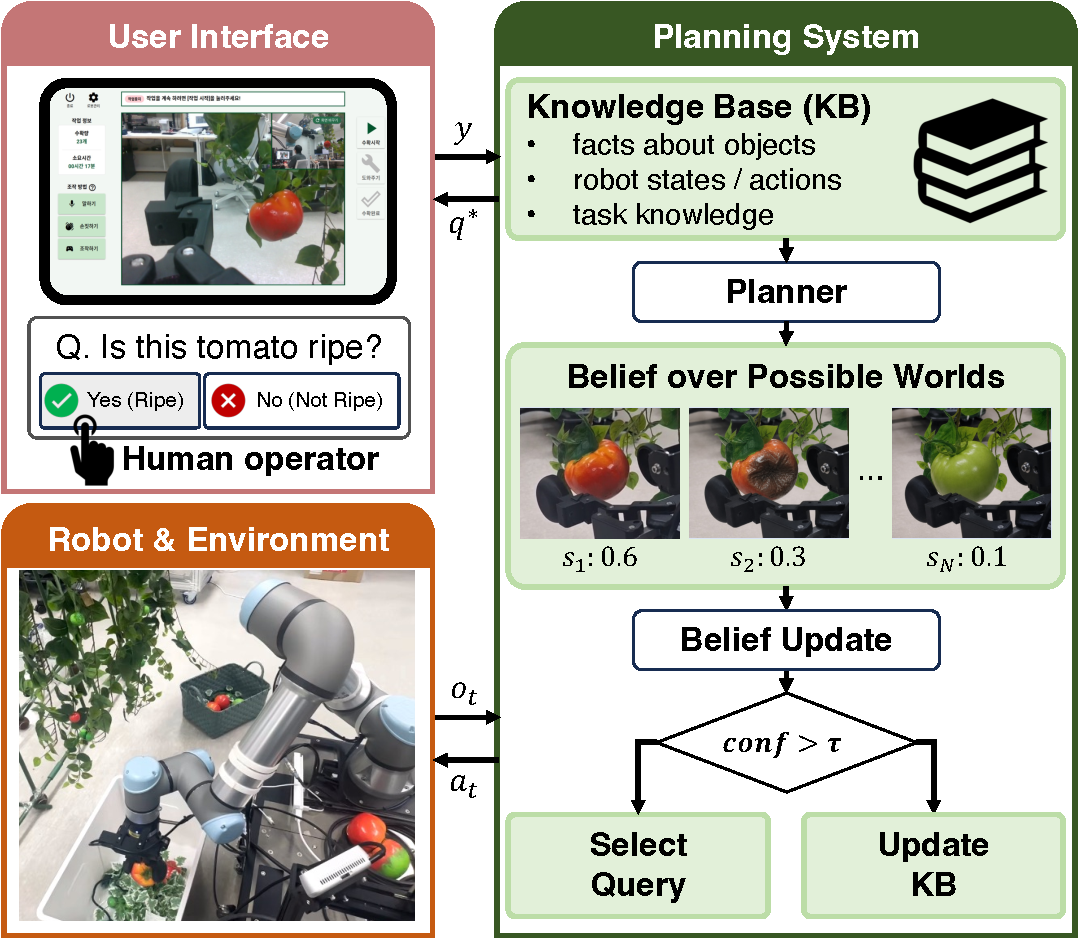
\includegraphics[width=0.995\linewidth]{figures/fig2_method.pdf}
\caption{Online planning and querying. If belief confidence falls below $\tau$, the robot queries the selected fact $q^*$ and uses the Boolean response $y\in\{\texttt{true},\texttt{false}\}$ to update the belief and knowledge base.}
\label{fig:pm}
\end{figure}







\subsubsection{What to Query}~\label{method:what}
If belief confidence falls below $\tau$, the robot triggers a query and must decide which fact to verify. Since verification eliminates state hypotheses that are inconsistent with the answer, we select the fact with the largest expected reduction in belief entropy.

\begin{algorithm}[t]
\caption{Planning and Querying}
\label{alg:online_planning}
\DontPrintSemicolon
\textbf{Input}\quad initial state $s_0^{K}$, goal condition $\mathcal{G}$, confidence threshold $\tau$, step limit $T_{\max}$\;
\textbf{Output}\quad executed action sequence $\pi$\;
\BlankLine
$\mathcal{B}\gets\{(s_0^{K},1)\}\qquad t\gets0\qquad \pi\gets()$\label{alg1_planning:initialize}\;
\While{$t<T_{\max}\land\mathcal{G}\nsubseteq s_t^{K}$}{
    \label{alg1_planning:termination}
    $a_t\gets$\Search{$\mathcal{B}$}\label{alg1_planning:search}\;
    \If{$a_t=\emptyset$}{
        \textbf{break}\label{alg1_planning:dead_end}\tcp*{dead end}
    }
    execute $a_t$ and receive $o_{t+1}$\label{alg1_planning:execute}\;
    $\pi\gets\pi\mathbin{\|}a_t$\label{alg1_planning:record}\;
    $\mathcal{B}\gets$\UpdateBelief{$s_t^{K},a_t,o_{t+1}$}\label{alg1_planning:belief_update}\;
    $c\gets\mathrm{Conf}(\mathcal{B})$\label{alg1_planning:compute_conf}\;
    \While{$c<\tau$}{
        $q^*\gets$\SelectBestHypothesis{$\mathcal{B}$}\label{alg1_planning:select_hypo}\;
        \If{$q^*=\emptyset$}{
            \textbf{break}\label{alg1_planning:no_candidate}\tcp*{no differentiating fact}
        }
        $y\gets$\QuerySource{$q^*$}\label{alg1_planning:query}\;
        $\mathcal{B}\gets$\FilterBelief{$\mathcal{B},q^*,y$}\label{alg1_planning:filter}\;
        $c\gets\mathrm{Conf}(\mathcal{B})$\label{alg1_planning:recompute_conf}\;
    }
    $s_{t+1}^{K}\gets\arg\max_{s^k\in\mathcal{B}}w_k$\label{alg1_planning:commit}\;
    $t\gets t+1$\label{alg1_planning:advance}\;
}
\KwRet $\pi$\label{alg1_planning:return}\;
\end{algorithm}



Specifically, we define the query candidate set $\mathcal{Q}(\mathcal{B})$ by extracting atomic facts whose truth values differ across the remaining frontier states in the belief,
\[\mathcal{Q}(\mathcal{B}) = \bigcup_{(s,w)\in\mathcal{B}}s \setminus \bigcap_{(s,w)\in\mathcal{B}}s.\]
For each candidate fact $q\in\mathcal{Q}(\mathcal{B})$, we partition the belief according to whether $q$ holds in each state,
\[
\begin{aligned}
\mathcal{B}^{q+}&=\{(s^k,w_k)\mid q\in s^k\},\\
\mathcal{B}^{q-}&=\{(s^k,w_k)\mid q\notin s^k\}.
\end{aligned}
\]
Let $P(q)=\sum_{k:q\in s^k}w_k$ and $P(\neg q)=1-P(q)$. Entropy within each subset is computed after conditionally normalizing its weights. The expected posterior entropy of asking about $q$ is
\[\mathbb{E}[\mathcal{H}\mid q] = P(q)\mathcal{H}(\mathcal{B}^{q+}) + P(\neg q)\mathcal{H}(\mathcal{B}^{q-}).\]
The selected query is
\begin{equation}~\label{eq:select_hypo}
q^* = \arg\min_{q\in\mathcal{Q}(\mathcal{B})} \left[P(q)\mathcal{H}(\mathcal{B}^{q+})+P(\neg q)\mathcal{H}(\mathcal{B}^{q-})\right].
\end{equation}
Eq.~\ref{eq:select_hypo} selects the fact $q^*$ that maximizes expected entropy reduction. The robot then converts this fact into a binary query about the current state. For example, $q^*=\texttt{ripe}(\text{tomato}_1)$ produces the question \textit{`Is tomato 1 ripe?'}. Based on the response $y\in\{\texttt{true},\texttt{false}\}$, the robot updates the belief by removing states inconsistent with the reported truth value,
\begin{equation}
\mathcal{B}
\leftarrow
\begin{cases}
\{(s^k,w_k)\mid q^*\in s^k\}, & y=\texttt{true},\\
\{(s^k,w_k)\mid q^*\notin s^k\}, & y=\texttt{false}.
\end{cases}
\label{eq:filter}
\end{equation}
The retained weights are renormalized, confidence is recomputed, and another fact is selected if confidence remains below $\tau$. The loop ends if the threshold is met or no differentiating fact remains. The robot then commits the maximum a posteriori state
\[s_{t+1}^{K} = \arg\max_{s^k\in\mathcal{B}_{t+1}}w_k \]
for subsequent symbolic planning.

Alg.~\ref{alg:online_planning} explains the overall online planning and querying procedure. The robot first initializes the belief, step counter, and action sequence (line~\ref{alg1_planning:initialize}). Execution continues while $t<T_{\max}$ and the goal condition is not satisfied, $\mathcal{G}\nsubseteq s_t^{K}$ (line~\ref{alg1_planning:termination}). At each step, POMCP selects an action (line~\ref{alg1_planning:search}), and execution stops if no action is available (line~\ref{alg1_planning:dead_end}). Otherwise, the robot executes the action  (lines~\ref{alg1_planning:execute} and~\ref{alg1_planning:record}), then constructs the weighted frontier belief and computes confidence (lines~\ref{alg1_planning:belief_update} and~\ref{alg1_planning:compute_conf}). If confidence falls below $\tau$, the robot selects a candidate fact (line~\ref{alg1_planning:select_hypo}). If no candidate remains, the query loop ends (line~\ref{alg1_planning:no_candidate}). Otherwise, the robot obtains an external response and filters the belief (lines~\ref{alg1_planning:query} and~\ref{alg1_planning:filter}), then recomputes confidence (line~\ref{alg1_planning:recompute_conf}). After the query loop, the most probable remaining state becomes the next symbolic planning state (line~\ref{alg1_planning:commit}). Appx.~\ref{appx:algorithms} provides the detailed POMCP search, simulation, and rollout procedures.



\subsection{System Implementation}~\label{method:modules}

\begin{figure*}[t]
\captionsetup{skip=0pt}
\centering
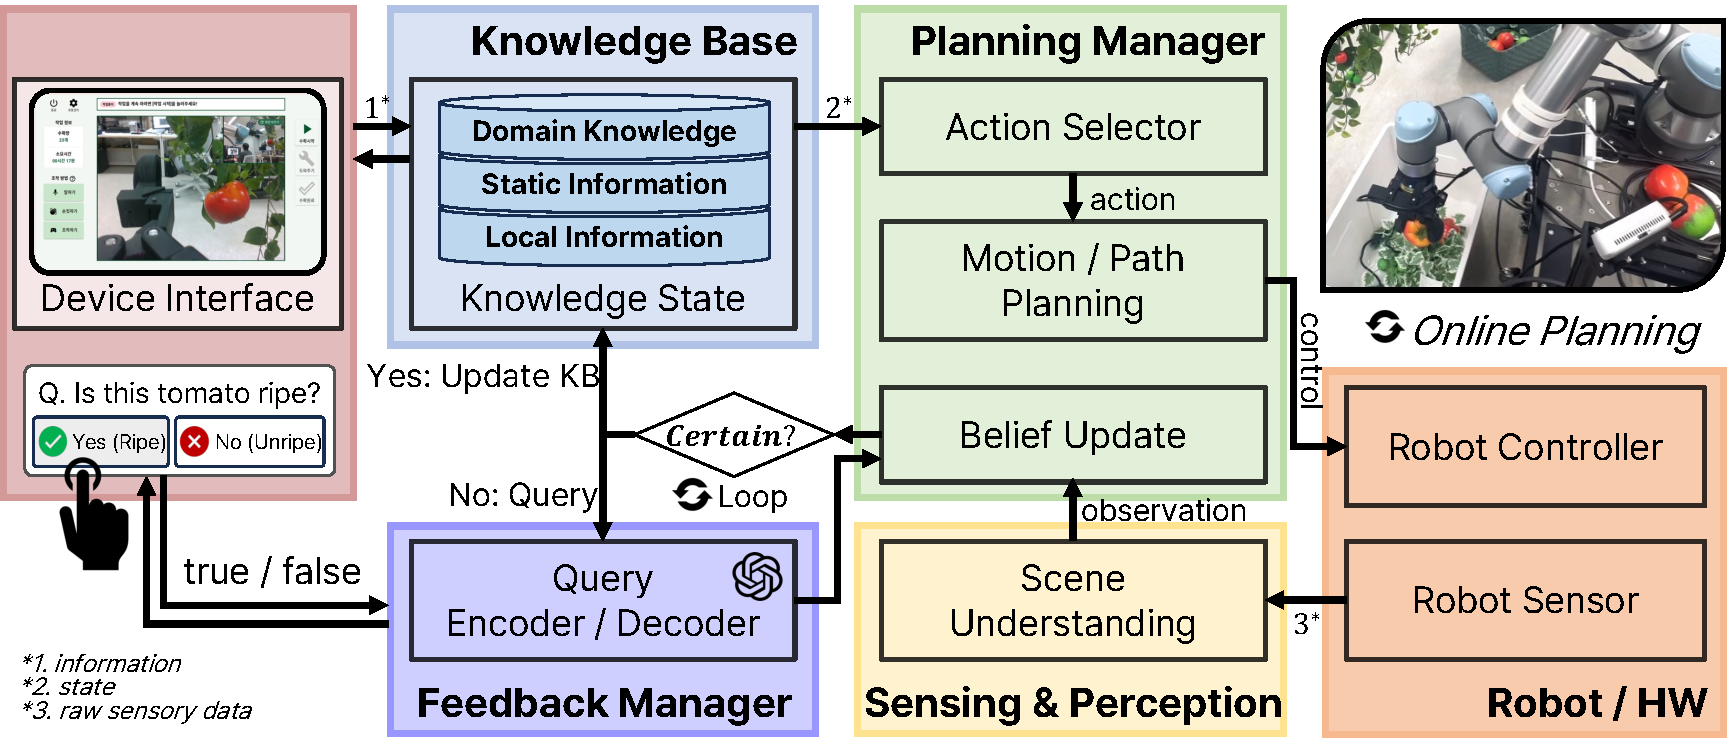
\includegraphics[width=0.98\linewidth]{figures/fig3_implementation.pdf}
\caption{Framework for robot execution of the proposed planning and querying method. The Knowledge Base (KB) stores shared symbolic facts and action models, while Sensing and Perception (SP) supplies observations from robot sensors. The Planning Manager (PM) selects actions and determines queries. If belief confidence falls below $\tau$, the Feedback Manager (FM) converts the selected fact into a question that the User Interface (UI) presents to the human. The FM converts the response into Boolean evidence, which the PM uses to update the belief and continue planning.}\label{fig:data_flow}
\end{figure*}

We implement a modular framework to execute the proposed planning and querying method on a robot, as shown in Fig.~\ref{fig:data_flow}. The Knowledge Base (KB) stores symbolic facts and action models, and Sensing and Perception (SP) provides observations and numeric state estimates from sensor data. The Planning Manager (PM) uses this information to select robot actions, construct the frontier belief, and decide when and what to query. The Feedback Manager (FM) converts the selected fact into a question and the response into evidence for the belief update. The User Interface (UI) presents the questions and collects responses during human interaction.

\label{method:KB}
The KB partitions information into domain knowledge $\mathcal{I}^{D}$, static structured information $\mathcal{I}^{S}$, and local information $\mathcal{I}^{L}$ obtained during execution. 
\[\mathcal{KB}=\mathcal{I}^{D}\sqcup\mathcal{I}^{S}\sqcup\mathcal{I}^{L}.\]\footnote{The symbol $\sqcup$ denotes the disjoint union, indicating that the three knowledge sets are treated as distinct components.}
Domain knowledge contains action schemas and task rules. Static information includes invariant facts and fixed map or robot parameters. Local information contains perceptual facts and numeric fluents that are updated during execution. SP maps raw sensor input to these task-level observations. For example, RGB-D sensing can update object pose and ripeness estimates, while the symbolic observation likelihood determines how those observations weight the frontier states.

\label{method:action_execution}
Each symbolic action invokes a robot skill. Actions such as $\texttt{navigate}(\text{robot},l_1,l_2)$ and $\texttt{pick}(\text{robot},\text{tomato}_1)$ specify task-level intentions, while an off-the-shelf motion planner such as MoveIt~\cite{chitta2012moveit} uses numeric fluents from the KB to generate low-level motion. This separation allows the feedback policy to operate on task-level facts without depending on a particular motion-planning implementation.

\label{method:FM}
The FM maps the selected predicate to a predefined question template and converts the response to a Boolean value. During human interaction, the tablet UI displays the camera view, highlights the referenced object with a bounding box, and presents simple response options. Participants answer questions about the displayed state fact, and the planner selects the next robot action.

\section{Experiments}~\label{experiment}
We evaluate our method in simulation and on physical robots. The evaluation covers waste sorting (\textit{Sort}) and tomato harvesting (\textit{Harvest}). We first compare the complete query policies in simulation with correct oracle responses. We then evaluate physical robot execution with responses from a VLM and human participants. Ablation experiments examine the contributions of query timing and query selection. A threshold sweep examines the balance between task success and query count.

The oracle experiments include $200$ trials per domain and condition. The VLM experiments include $40$ trials per domain and method. The planned human evaluation is designed for five participants with $10$ trials per domain and method for a total of $40$ trials.

\begin{figure}[t]
    \centering
    \begin{subfigure}[t]{0.48\linewidth}
        \centering
        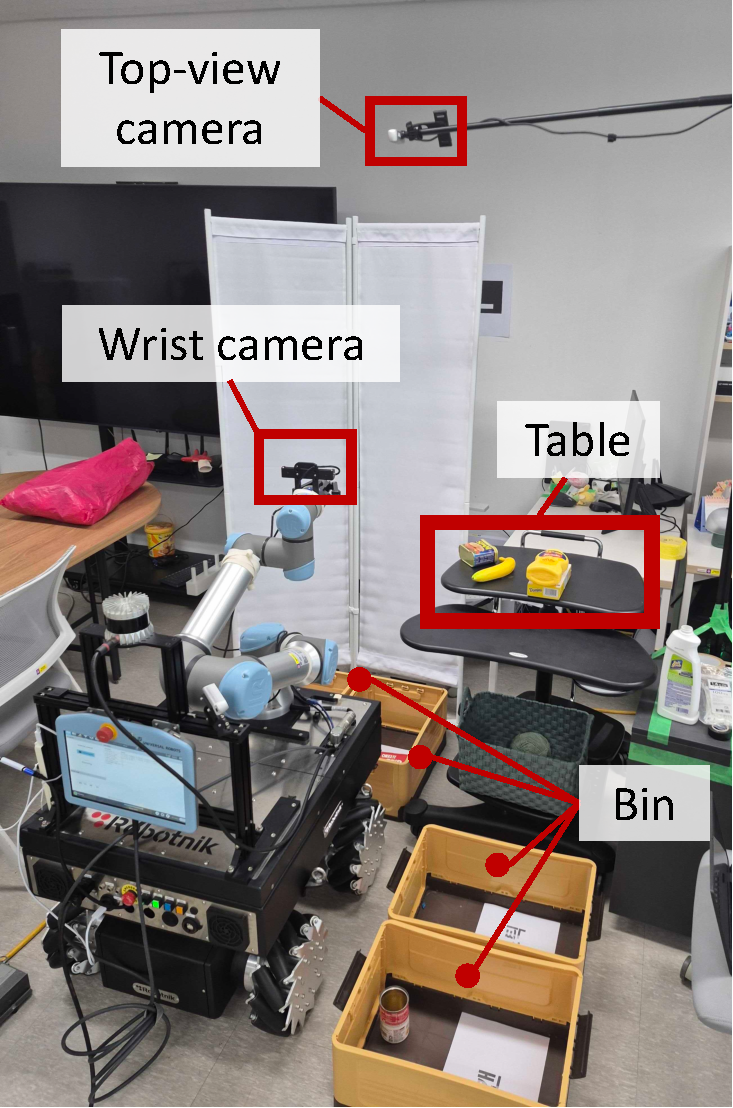
\includegraphics[width=\linewidth]{figures/03_SETUP/01_WasteSortingEnv.pdf}
        \caption{Sort}
        \label{fig:dom1}
    \end{subfigure}\hfill
    \begin{subfigure}[t]{0.48\linewidth}
        \centering
        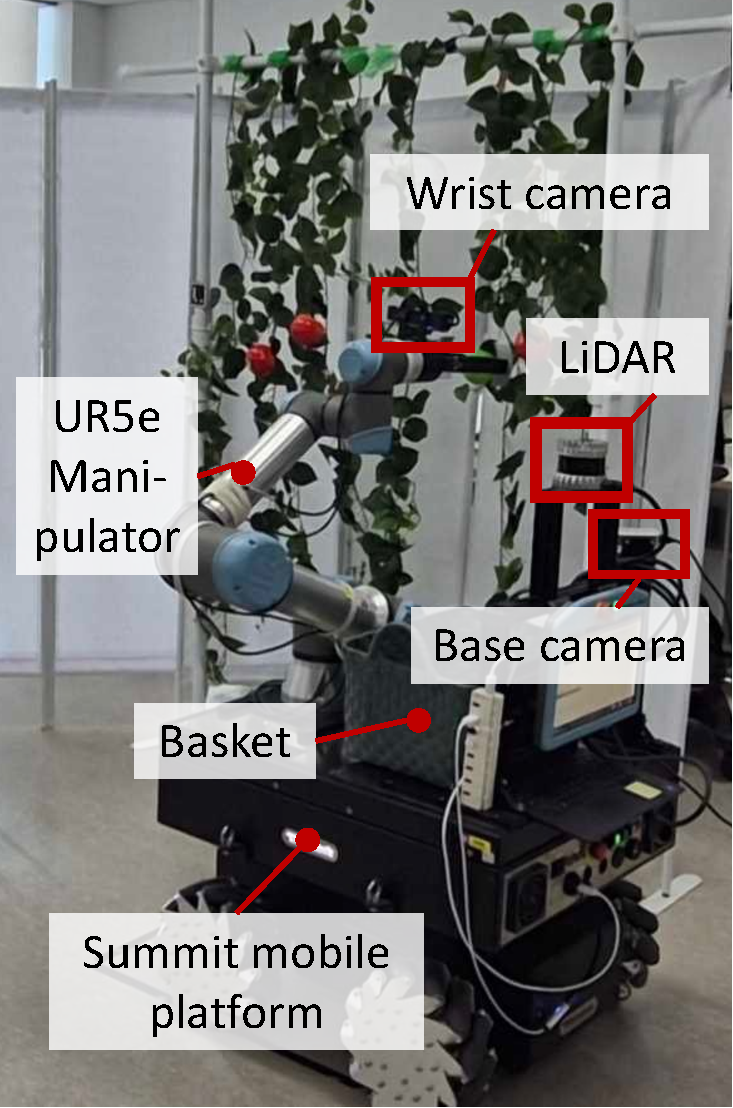
\includegraphics[width=\linewidth]{figures/03_SETUP/02_TomatoHarvestEnv.pdf}
        \caption{Harvest}
        \label{fig:dom2}
    \end{subfigure}
\caption{Physical robot setups for the two task domains. (a) Sort uses a fixed UR5e arm to sort objects into the appropriate bins. (b) Harvest uses a Summit mobile platform with a UR5e arm to navigate between tomato stems and harvest tomatoes. Annotations identify robot components, sensors, and task equipment.}    \label{fig:env_setting}
\end{figure}


\subsection{Experimental Setup}~\label{exp:setup}
The oracle experiments use simulated task execution and exact external responses. The VLM and human experiments use physical robots in laboratory environments. Fig.~\ref{fig:env_setting} shows the physical setups. Sort uses a fixed UR5e robot arm. Harvest uses a Summit mobile platform equipped with a UR5e robot arm. The mobile platform uses an RGB-D camera for perception and LiDAR for localization. Sort uses SAM3 for object detection~\citep{carion2025sam3segmentconcepts}. Harvest uses YOLOv12 for object detection~\citep{tian2025yolov12}.


% \subsubsection{Task Domains}~\label{exp:setup_domains}
% The Sort task requires the robot to place every object in the correct bin. The UR5e robot is positioned between the objects and recycling bins in Fig.~\ref{fig:dom1}. All objects are within reach. The robot can detect objects and then pick and place them. Each object belongs to one of four waste categories corresponding to general waste or recyclable paper or cans or plastic. The categories are initially unknown. The main sources of uncertainty in this domain are occlusion and noisy sensor observations. In simulation we randomize the initial object arrangement for each trial. A trial succeeds if the robot places all objects in the correct bins within the step limit. Each correct placement yields a task reward of $+5$. Completion of the task yields an additional reward of $+10$. A penalty of $-10$ applies to the third and each subsequent detection action in a consecutive sequence.

% The Harvest task requires the robot to harvest fresh ripe tomatoes and discard rotten tomatoes. Four tomatoes are distributed across two stems in Fig.~\ref{fig:dom2}. The robot navigates between the docking station and the two stems. The \texttt{detect} action distinguishes ripe from unripe tomatoes. After a tomato is picked the \texttt{scan} action distinguishes fresh from rotten tomatoes. The robot uses \texttt{place} for fresh tomatoes and \texttt{discard} for rotten tomatoes. Unripe tomatoes remain on the stem. The main source of uncertainty in this domain is noisy sensor observations. In simulation we randomize tomato locations across the two stems for each trial. A trial succeeds if all fresh ripe tomatoes are harvested and all rotten tomatoes are discarded within the step limit. Correct placement of a fresh tomato or disposal of a rotten tomato yields a task reward of $+10$. Consecutive \texttt{detect} actions at the same stem and consecutive \texttt{scan} actions on the same tomato incur a penalty of $-5$ from the second action onward.


\subsubsection{Task Domains}~\label{exp:setup_domains}
We evaluate two domains with different sources of uncertainty (Fig.~\ref{fig:env_setting}). In Sort, the robot detects, picks, and places objects into bins for four waste categories. Object categories are initially unknown, and occlusion and noisy observations create uncertainty about object presence and category. In Harvest, the robot navigates between two stems to harvest fresh ripe tomatoes and discard rotten ones, leaving unripe tomatoes untouched. Detection estimates ripeness, while scanning after picking distinguishes fresh from rotten tomatoes. Noisy observations create uncertainty about tomato state.



\subsubsection{Implementation Details}~\label{exp:details}
Our POMCP planner uses $100$ simulations per planning step with a maximum simulation depth of $20$. The discount factor is $\gamma=0.2$ and the UCB exploration constant is $c=1.0$. The default confidence threshold is $\tau=0.8$. We use Gemma 4 31B IT with NVFP4 quantization~\citep{gemmateam2026gemma4} as the external expert in the VLM experiments. Appendix~\ref{appx:settings} provides the baseline configurations and additional experimental details.

\subsubsection{Evaluation Metrics}~\label{exp:metrics}
Success rate is the fraction of all trials that achieve the task goal within the trial limit. Query count is the number of external requests per trial. Query probability is the fraction of physical steps that trigger at least one query. Plan length is the number of physical actions executed per trial. Search time is the cumulative time spent on plan search per trial. Interaction time is the cumulative time spent on external requests and response processing per trial. We report interaction time only for the VLM and human experiments.

% Numerical reference is the manuscript summary in experiments_final/04_Total_Summary.
\subsection{System Evaluation}~\label{exp:sys_eval}

\begin{table*}[t]
\centering
\caption{Query timing and query selection strategies. Columns indicate query timing criteria and rows indicate query selection criteria. KnowNo and IntroPlan and Query-Action are the baselines. Fully-Random and Q1--Q2 and W1--W3 are the ablation configurations. Ours serves as the reference method for both comparisons. A dash denotes a combination not evaluated in this study.}
\label{tab:query_strategy_matrix}
\small
\newcommand{\queryhighlight}[2]{%
    \tikz[baseline=(marker.base)]{%
        \node[inner xsep=3pt,inner ysep=1pt] (marker) {\phantom{#2}};
        \fill[#1,opacity=0.7]
            ([xshift=-1pt,yshift=-0.5pt]marker.south west) --
            ([xshift=1pt,yshift=0.5pt]marker.south east) --
            ([xshift=2pt,yshift=-0.5pt]marker.north east) --
            ([xshift=0.5pt,yshift=0.5pt]marker.north west) -- cycle;
        \node[inner xsep=3pt,inner ysep=1pt] at (marker.center) {#2};
    }%
}
\begin{tabular}{lcccc}
\toprule
\diagbox[width=2.6cm,height=0.75cm,dir=NW,linewidth=0.3pt]{What}{When} & Random & Conformal Prediction & Reward-based & Confidence \\
\midrule
Random & \queryhighlight{blue!25}{Fully-Random} & -- & -- & \queryhighlight{blue!25}{Q1} \\
Conformal Set & -- & \queryhighlight{yellow!65}{KnowNo}, \queryhighlight{yellow!65}{IntroPlan} & -- & -- \\
Reward-based & -- & -- & \queryhighlight{yellow!65}{Query-Action} & \queryhighlight{blue!25}{Q2} \\
Entropy Gain & \queryhighlight{blue!25}{W1} & \queryhighlight{blue!25}{W2} & \queryhighlight{blue!25}{W3} & \queryhighlight{green!35}{\textbf{Ours}} \\
\bottomrule
\end{tabular}
\end{table*}

Table~\ref{tab:query_strategy_matrix} summarizes the baseline and ablation configurations. The baseline comparison in Sec.~\ref{exp:sys_baseline} evaluates KnowNo, IntroPlan, and Query-Action against Ours. The baseline evaluation covers oracle responses in simulation and VLM and human responses during physical execution. The ablation study in Sec.~\ref{exp:policy_ablation} evaluates Fully-Random, Q1--Q2, and W1--W3 against Ours where W1--W3 examine query timing (when) and Q1--Q2 examine query selection (what). Finally the threshold study in Sec.~\ref{exp:sys_threshold} examines how the confidence threshold affects task success and query count. Both the ablation and threshold studies use oracle responses in simulation.



\subsubsection{Baseline Comparison}~\label{exp:sys_baseline}

\noindent\textbf{Oracle}. The oracle comparison includes three baselines with the query timing and selection strategies summarized in Table~\ref{tab:query_strategy_matrix}. KnowNo~\cite{ren2023robots} requests an action choice if its conformal prediction set does not specify a single ordinary action. IntroPlan~\cite{liang2024introspective} extends KnowNo and incorporates retrieved examples and explanations into candidate evaluation before it requests an action choice. Query-Action follows the standard POMDP approach to information gathering~\cite{kaelbling1998planning}. It includes Boolean state queries in the POMCP action space and selects them according to expected cumulative reward. Table~\ref{tab:baseline_results} and Fig.~\ref{fig:baseline_results} compare the four methods. 

\begin{figure*}[!tp]
\centering
\begin{subfigure}[t]{0.247\textwidth}
\centering
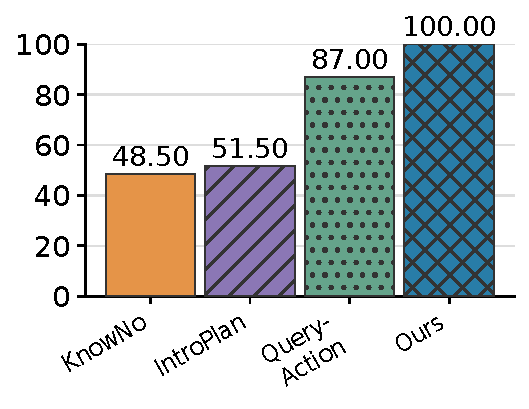
\includegraphics[width=\linewidth,height=.16\textheight,keepaspectratio]{figures/04_ORACLE_BASELINE/exp_oracle_waste_success.pdf}
\caption{W.S. Success rate (\%).}
\label{fig:baseline_oracle_waste_success}
\end{subfigure}%
\hspace{0.004\textwidth}%
\begin{subfigure}[t]{0.247\textwidth}
\centering
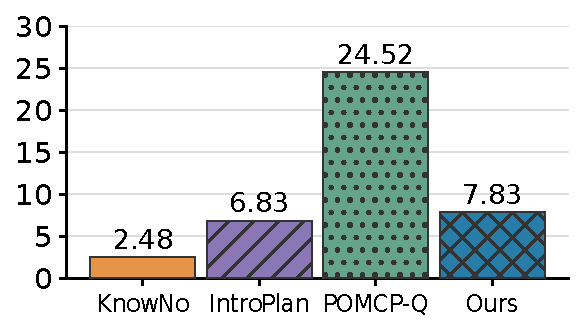
\includegraphics[width=\linewidth,height=.16\textheight,keepaspectratio]{figures/04_ORACLE_BASELINE/exp_oracle_waste_queries.pdf}
\caption{W.S. Query count.}
\label{fig:baseline_oracle_waste_queries}
\end{subfigure}%
\hspace{0.004\textwidth}%
\begin{subfigure}[t]{0.247\textwidth}
\centering
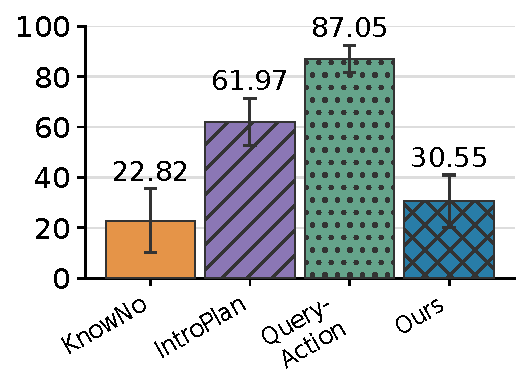
\includegraphics[width=\linewidth,height=.16\textheight,keepaspectratio]{figures/04_ORACLE_BASELINE/exp_oracle_waste_query_probability.pdf}
\caption{W.S. Query prob. (\%).}
\label{fig:baseline_oracle_waste_query_probability}
\end{subfigure}%
\hspace{0.004\textwidth}%
\begin{subfigure}[t]{0.247\textwidth}
\centering
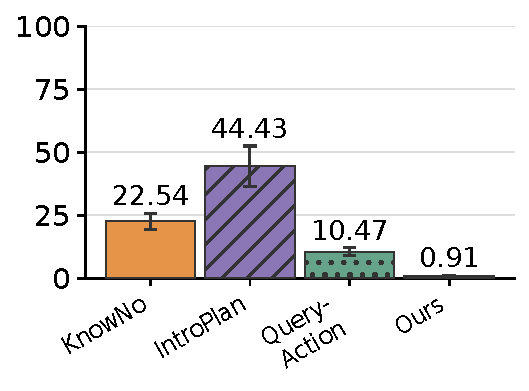
\includegraphics[width=\linewidth,height=.16\textheight,keepaspectratio]{figures/04_ORACLE_BASELINE/exp_oracle_waste_plan_time.pdf}
\caption{W.S. Plan time (s).}
\label{fig:baseline_oracle_waste_plan_time}
\end{subfigure}
\par\smallskip
\begin{subfigure}[t]{0.247\textwidth}
\centering
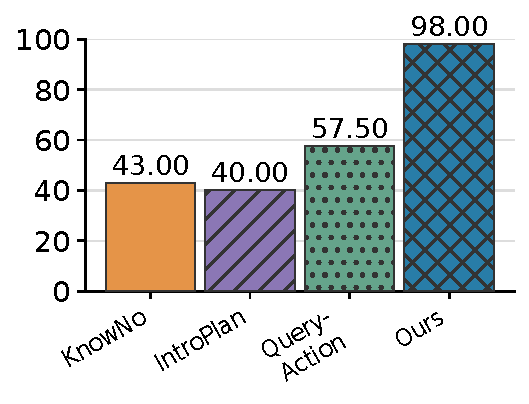
\includegraphics[width=\linewidth,height=.16\textheight,keepaspectratio]{figures/04_ORACLE_BASELINE/exp_oracle_tomato_success.pdf}
\caption{T.H. Success rate (\%).}
\label{fig:baseline_oracle_tomato_success}
\end{subfigure}%
\hspace{0.004\textwidth}%
\begin{subfigure}[t]{0.247\textwidth}
\centering
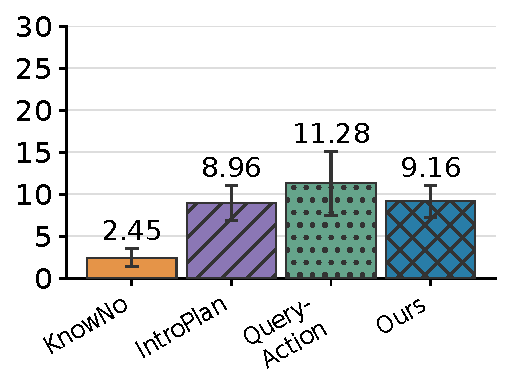
\includegraphics[width=\linewidth,height=.16\textheight,keepaspectratio]{figures/04_ORACLE_BASELINE/exp_oracle_tomato_queries.pdf}
\caption{T.H. Query count.}
\label{fig:baseline_oracle_tomato_queries}
\end{subfigure}%
\hspace{0.004\textwidth}%
\begin{subfigure}[t]{0.247\textwidth}
\centering
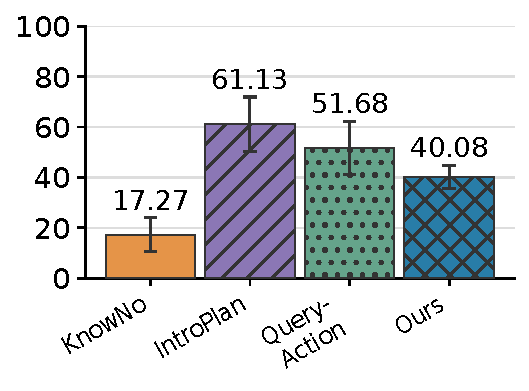
\includegraphics[width=\linewidth,height=.16\textheight,keepaspectratio]{figures/04_ORACLE_BASELINE/exp_oracle_tomato_query_probability.pdf}
\caption{T.H. Query prob. (\%).}
\label{fig:baseline_oracle_tomato_query_probability}
\end{subfigure}%
\hspace{0.004\textwidth}%
\begin{subfigure}[t]{0.247\textwidth}
\centering
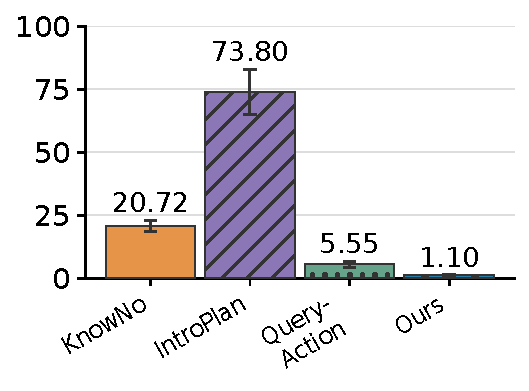
\includegraphics[width=\linewidth,height=.16\textheight,keepaspectratio]{figures/04_ORACLE_BASELINE/exp_oracle_tomato_plan_time.pdf}
\caption{T.H. Plan time (s).}
\label{fig:baseline_oracle_tomato_plan_time}
\end{subfigure}
\caption{Oracle baseline comparison. (a)--(d) show success rate, query count, query probability, and plan time for WasteSorting (short for W.S.). (e)--(h) show the same metrics for TomatoHarvesting (short for T.H.) in the same order. Across both domains, our method achieves the highest success rate and the lowest plan time. These results suggest that effective query timing and selection are more important than query count alone for reliable task execution.}
\label{fig:baseline_results}
\end{figure*}


\begin{table*}[t]
\centering
\caption{Oracle baseline comparison results by domain. Bold values indicate the highest success rate and the lowest query count, query probability, and plan length within each domain.}
\label{tab:baseline_results}
\small
\setlength{\tabcolsep}{4pt}
\begin{tabular*}{\textwidth}{@{\extracolsep{\fill}}llcccc}
% \begin{tabular}{llcccc}
\toprule
Domain & Method & Success (\%) & Query count & \shortstack{Query prob.(\%)} & Plan length \\
\midrule
WasteSorting & KnowNo & 48.50 & $\boldsymbol{2.48 \pm 1.42}$ & $\boldsymbol{22.82 \pm 12.61}$ & $10.78 \pm 1.35$ \\
 & IntroPlan & 51.50 & $6.83 \pm 1.53$ & $61.97 \pm 9.35$ & $10.99 \pm 1.49$ \\
 & Query-Action & 87.00 & $24.52 \pm 5.39$ & $87.05 \pm 5.28$ & $11.89 \pm 1.53$ \\
 & Ours & \textbf{100.00} & $7.83 \pm 2.16$ & $30.55 \pm 10.41$ & $\boldsymbol{10.35 \pm 0.88}$ \\
\midrule
TomatoHarvesting & KnowNo & 43.00 & $\boldsymbol{2.45 \pm 1.06}$ & $\boldsymbol{17.27 \pm 6.67}$ & $14.01 \pm 1.07$ \\
 & IntroPlan & 40.00 & $8.96 \pm 2.04$ & $61.13 \pm 10.77$ & $14.61 \pm 1.46$ \\
 & Query-Action & 57.50 & $11.28 \pm 3.78$ & $51.68 \pm 10.45$ & $14.94 \pm 1.70$ \\
 & Ours & \textbf{98.00} & $9.16 \pm 1.90$ & $40.08 \pm 4.56$ & $\boldsymbol{13.97 \pm 1.15}$ \\
\bottomrule
\end{tabular*}
\end{table*}


As shown in Table~\ref{tab:baseline_results} and Fig.~\ref{fig:baseline_results}, our method achieves the highest success rate in both domains. It completes all $200$ WasteSorting trials and $196$ of $200$ TomatoHarvesting trials. Our method achieves success rates of $100.00\%$ in WasteSorting and $98.00\%$ in TomatoHarvesting compared with $87.00\%$ and $57.50\%$ for Query-Action. The mean query counts are also lower at $7.83$ and $9.16$ compared with $24.52$ and $11.28$ for Query-Action. Two factors may explain the lower success rate and higher query count of Query-Action. First, query actions expand the action space so POMCP must evaluate more alternatives within the same simulation budget. Second, expected task reward does not explicitly measure confidence in the current state. Our method selects queries at the observation stage and restricts POMCP planning to physical actions. These results show that a higher query count alone does not guarantee a higher success rate.

Compared to KnowNo and IntroPlan, our method uses more queries. Their mean query counts are $2.48$ and $6.83$ in WasteSorting compared with $7.83$ for our method. In TomatoHarvesting, the corresponding counts are $2.45$ and $8.96$ compared with $9.16$ for our method. This difference in query count arises from how each method handles a query trigger. If a query is triggered, our method repeats queries until belief confidence reaches $\tau$. KnowNo and IntroPlan ask only one question per trigger. Therefore our method can use more queries despite a lower query probability than IntroPlan. However KnowNo and IntroPlan achieve success rates of only $48.50\%$ and $51.50\%$ in WasteSorting and $43.00\%$ and $40.00\%$ in TomatoHarvesting. Therefore a system is not necessarily better simply because it uses fewer queries.

Plan time is also lowest for Ours in both domains despite the additional queries compared with KnowNo and IntroPlan. In WasteSorting, mean plan time is $0.91$ seconds for Ours compared with $22.54$ seconds for KnowNo, $44.43$ seconds for IntroPlan, and $10.47$ seconds for Query-Action. In TomatoHarvesting, the corresponding values are $1.10$, $20.72$, $73.80$, and $5.55$ seconds. KnowNo and IntroPlan require language-model inference for candidate generation and scoring at each planning step. IntroPlan performs additional reasoning and candidate evaluation, which increases inference time compared with KnowNo. Ours evaluates query timing and selection from the belief state and searches only over physical actions. The smaller search space supports faster planning than Query-Action. The time comparisons suggest that belief-based search can reduce planning time without repeated language-model inference. % Therefore a higher query count does not necessarily imply a higher planning cost.

Our method combines confidence-based query timing with entropy gain query selection and achieves the highest success rate in both domains. The baseline comparisons suggest that effective query timing and selection are more important than query count alone.

\noindent\textbf{VLM}\label{exp:vlm_eval}. We evaluate whether the trends in task success and query behavior from the oracle experiments also hold in a real-world setting. We first prompt a VLM to act as an external expert and evaluate query policies on physical robots.\footnote{Appendix~\ref{appx:vlm_prompts} provides the VLM prompts.} We select KnowNo as the baseline because it achieves a high success rate relative to its query count in the oracle experiments. Each method has $40$ trials per domain. Fig.~\ref{fig:vlm_results} presents the VLM results.

\begin{figure*}[!tp]
\centering
\begin{subfigure}[t]{0.247\textwidth}
\centering
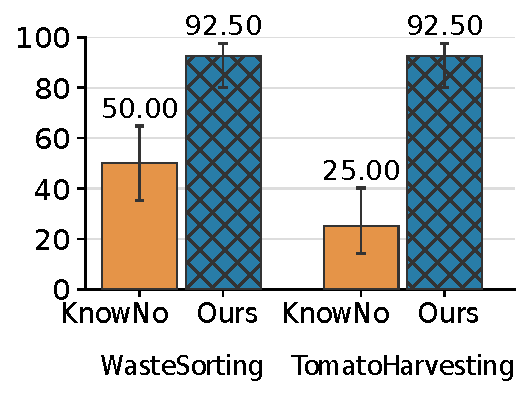
\includegraphics[width=\linewidth,height=.20\textheight,keepaspectratio]{figures/05_VLM_BASELINE/exp_vlm_success.pdf}
\caption{Success rate (\%).}
\label{fig:vlm_vlm_success}
\end{subfigure}%
\hspace{0.004\textwidth}%
\begin{subfigure}[t]{0.247\textwidth}
\centering
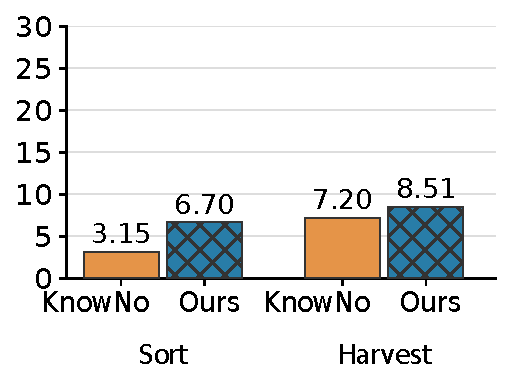
\includegraphics[width=\linewidth,height=.20\textheight,keepaspectratio]{figures/05_VLM_BASELINE/exp_vlm_queries.pdf}
\caption{Query count.}
\label{fig:vlm_vlm_queries}
\end{subfigure}%
\hspace{0.004\textwidth}%
\begin{subfigure}[t]{0.247\textwidth}
\centering
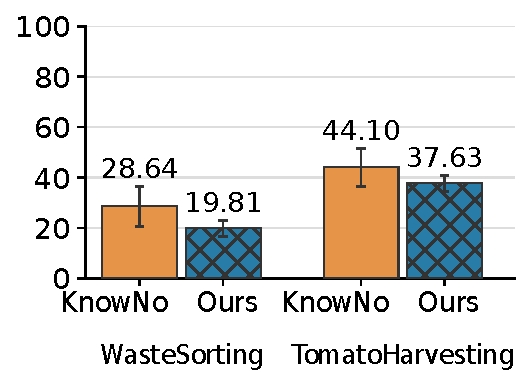
\includegraphics[width=\linewidth,height=.20\textheight,keepaspectratio]{figures/05_VLM_BASELINE/exp_vlm_query_probability.pdf}
\caption{Query probability (\%).}
\label{fig:vlm_vlm_query_probability}
\end{subfigure}%
\hspace{0.004\textwidth}%
\begin{subfigure}[t]{0.247\textwidth}
\centering
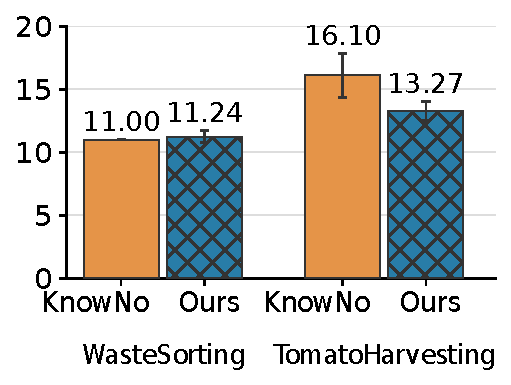
\includegraphics[width=\linewidth,height=.20\textheight,keepaspectratio]{figures/05_VLM_BASELINE/exp_vlm_plan_length.pdf}
\caption{Plan length.}
\label{fig:vlm_vlm_plan_length}
\end{subfigure}
\par\smallskip
\begin{subfigure}[t]{0.247\textwidth}
\centering
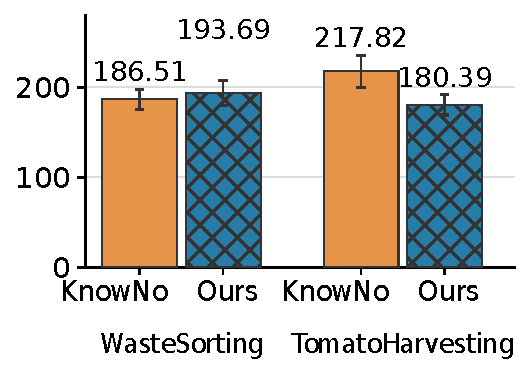
\includegraphics[width=\linewidth,height=.20\textheight,keepaspectratio]{figures/05_VLM_BASELINE/exp_vlm_total_time.pdf}
\caption{Total time (s).}
\label{fig:vlm_vlm_total_time}
\end{subfigure}%
\hspace{0.004\textwidth}%
\begin{subfigure}[t]{0.247\textwidth}
\centering
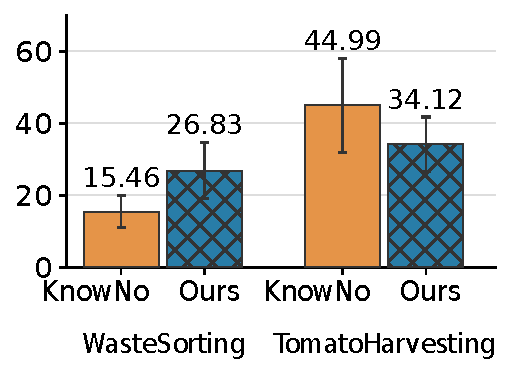
\includegraphics[width=\linewidth,height=.20\textheight,keepaspectratio]{figures/05_VLM_BASELINE/exp_vlm_interaction_time.pdf}
\caption{Interaction time (s).}
\label{fig:vlm_vlm_interaction_time}
\end{subfigure}%
\hspace{0.004\textwidth}%
\begin{subfigure}[t]{0.247\textwidth}
\centering
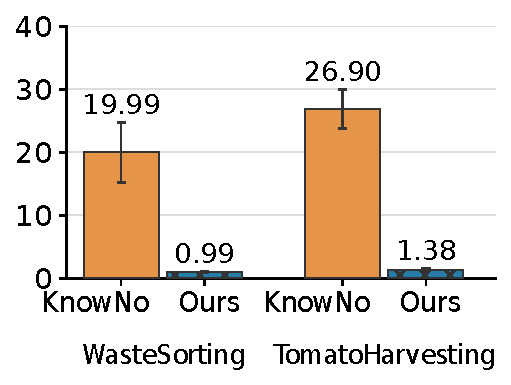
\includegraphics[width=\linewidth,height=.20\textheight,keepaspectratio]{figures/05_VLM_BASELINE/exp_vlm_planning_time.pdf}
\caption{Planning time (s).}
\label{fig:vlm_vlm_planning_time}
\end{subfigure}
\caption{Physical robot evaluation with VLM responses. (a)--(d) show success rate, query count, query probability, and plan length for both domains. (e)--(g) show total time, interaction time, and planning time for both domains. Across both domains, our method achieves higher success rates and shorter planning times than KnowNo despite more queries.}
\label{fig:vlm_results}
\end{figure*}



\begin{table*}[t]
\centering
\caption{Physical robot results with VLM and human responses. Parentheses give successful trials over all trials. Other metrics report means over successful trials. A dash marks human results that are not yet available.}
\label{tab:physical_robot_results}
\small
\setlength{\tabcolsep}{2.5pt}
\begin{tabular*}{\textwidth}{@{\extracolsep{\fill}}lllccccccc}
\toprule
Source & Domain & Method & Success (\%) & \shortstack{Query\\count} & \shortstack{Query\\prob. (\%)} & \shortstack{Plan\\length} & \shortstack{Total\\time (s)} & \shortstack{Interaction\\time (s)} & \shortstack{Planning\\time (s)} \\
\midrule
VLM & W.S. & KnowNo & 50.00 (20/40) & 3.15 & 28.64 & 11.00 & 186.51 & 15.46 & 20.08 \\
 &  & Ours & 92.50 (37/40) & 6.70 & 19.81 & 11.24 & 193.69 & 26.83 & 1.11 \\
\addlinespace
 & T.H. & KnowNo & 25.00 (10/40) & 7.20 & 44.10 & 16.10 & 217.82 & 44.99 & 27.68 \\
 &  & Ours & 92.50 (37/40) & 8.51 & 37.63 & 13.27 & 180.39 & 34.12 & 1.48 \\
\midrule
Human & W.S. & KnowNo & - (-/10) & - & - & - & - & - & - \\
 &  & Ours & - (-/10) & - & - & - & - & - & - \\
\addlinespace
 & T.H. & KnowNo & - (-/10) & - & - & - & - & - & - \\
 &  & Ours & - (-/10) & - & - & - & - & - & - \\
\bottomrule
\end{tabular*}
\end{table*}

Ours achieves a success rate of $92.50\%$ in both domains with VLM responses. KnowNo achieves $50.00\%$ in WasteSorting and $25.00\%$ in TomatoHarvesting. Mean query counts are $6.70$ for Ours and $3.15$ for KnowNo in WasteSorting and $8.51$ and $7.20$ in TomatoHarvesting. Consistent with the oracle experiments, Ours requires less search time than KnowNo. Mean search time is $0.99$ seconds for Ours and $19.99$ seconds for KnowNo in WasteSorting and $1.38$ and $26.90$ seconds in TomatoHarvesting. In TomatoHarvesting, interaction time and total time are $44.99$ and $217.82$ seconds for KnowNo compared with $34.12$ and $180.39$ seconds for Ours. Notably, KnowNo uses only $15.43\%$ fewer queries than Ours in TomatoHarvesting with VLM responses compared with $73.22\%$ fewer queries in the oracle experiments. However the similar query counts do not translate into similar execution costs. KnowNo executes longer plans, with $16.10$ physical actions compared with $13.27$ for Ours. Interaction time and total time for KnowNo are $31.86\%$ and $20.75\%$ longer than for Ours respectively.

To understand the differences from the oracle results, we analyze failed trials and distinguish VLM response errors from baseline planner failures. In WasteSorting, all three failures of Ours involve VLM feedback. For example, the VLM rejects a can classification from perception and the robot places the object in the plastic bin. KnowNo has three VLM response failures ($15\%$) and $17$ planner failures ($85\%$). The planner failures occur because KnowNo selects actions without requesting assistance despite unmet action preconditions. In TomatoHarvesting, all three failures of Ours also involve VLM feedback. KnowNo has $18$ VLM failures ($60\%$) and $12$ planner failures ($40\%$). The planner failures occur after action selections without external assistance. In six trials, the VLM repeatedly selects detection despite feasible alternatives and the robot reaches the step limit. The remaining $12$ VLM failures involve incorrect action selections.

The WasteSorting failures show that a single predicted action can still require additional state verification before execution. In TomatoHarvesting, action selection requires the VLM to reason about robot location and object states to determine the next action. The spatial reasoning burden can lead to less effective action choices. Even successful trials can then require additional queries and longer plans and more total time. Therefore fewer queries do not necessarily reduce interaction time or total time. Ours asks the VLM to verify current state facts and assigns action selection to the planner. The VLM assesses current observations with less need to reason about future actions and outcomes. Performance may also depend on what the VLM is asked to judge.




\begin{figure}[t]
\centering
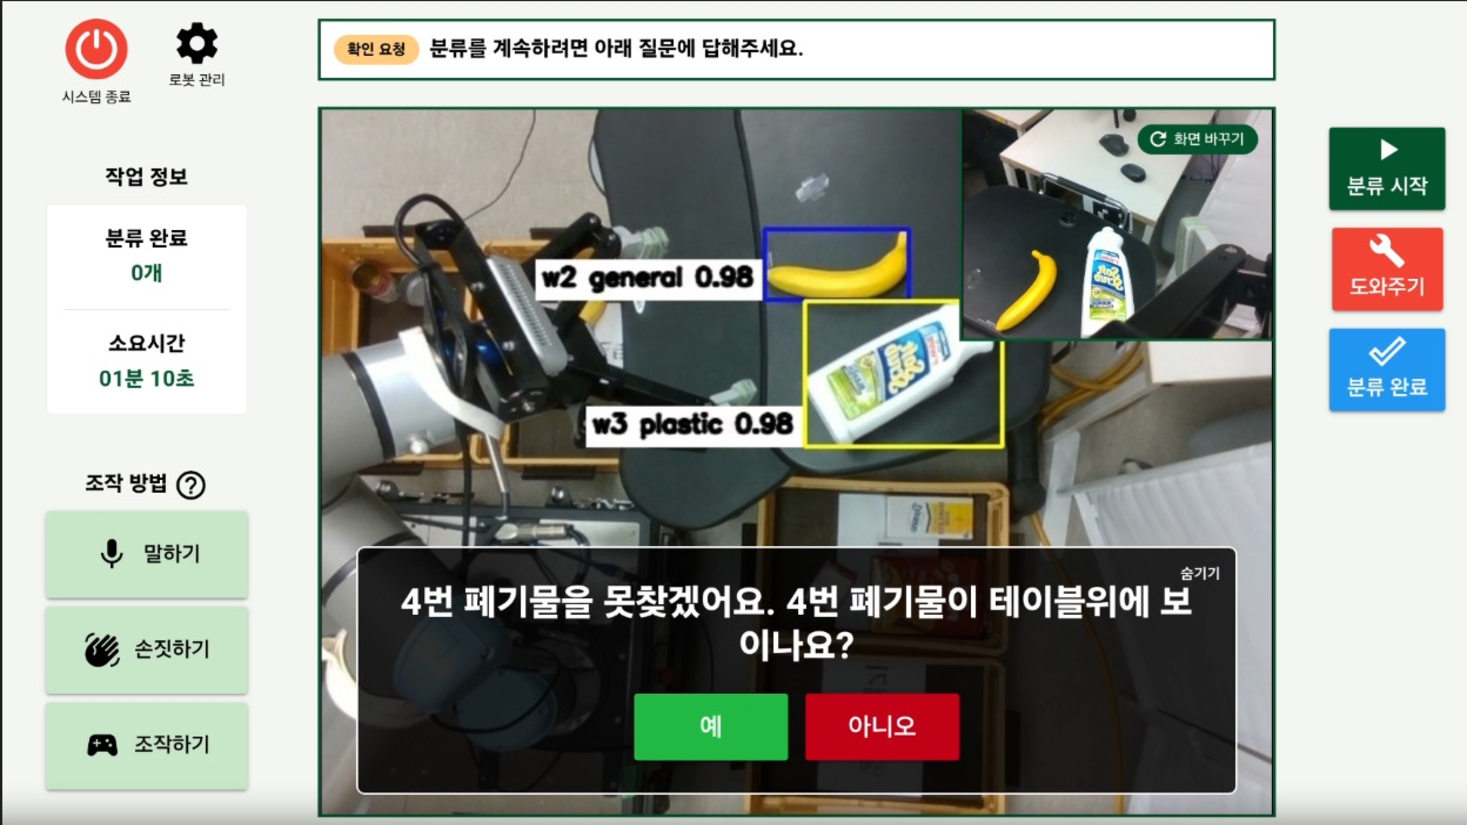
\includegraphics[width=\linewidth]{figures/exp_human_ui.pdf}
\caption{Tablet interface used in the human evaluation. Participants view the robot camera feeds and select responses to robot queries.}
\label{fig:human_tablet_interface}
\end{figure}


\begin{figure*}[!tp]
\centering
\begin{subfigure}[t]{0.247\textwidth}
\centering
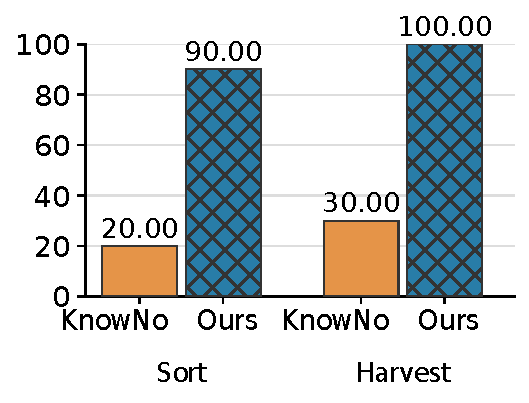
\includegraphics[width=\linewidth,height=.20\textheight,keepaspectratio]{figures/06_HUMAN_BASELINE/exp_human_success.pdf}
\caption{Success rate (\%).}
\label{fig:human_human_success}
\end{subfigure}%
\hspace{0.004\textwidth}%
\begin{subfigure}[t]{0.247\textwidth}
\centering
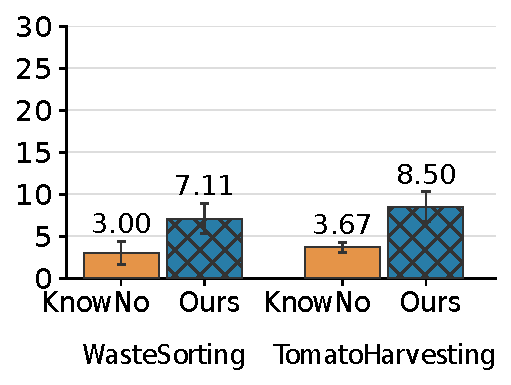
\includegraphics[width=\linewidth,height=.20\textheight,keepaspectratio]{figures/06_HUMAN_BASELINE/exp_human_queries.pdf}
\caption{Query count.}
\label{fig:human_human_queries}
\end{subfigure}%
\hspace{0.004\textwidth}%
\begin{subfigure}[t]{0.247\textwidth}
\centering
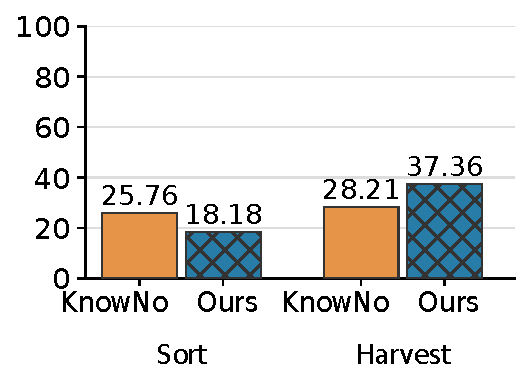
\includegraphics[width=\linewidth,height=.20\textheight,keepaspectratio]{figures/06_HUMAN_BASELINE/exp_human_query_probability.pdf}
\caption{Query probability (\%).}
\label{fig:human_human_query_probability}
\end{subfigure}%
\hspace{0.004\textwidth}%
\begin{subfigure}[t]{0.247\textwidth}
\centering
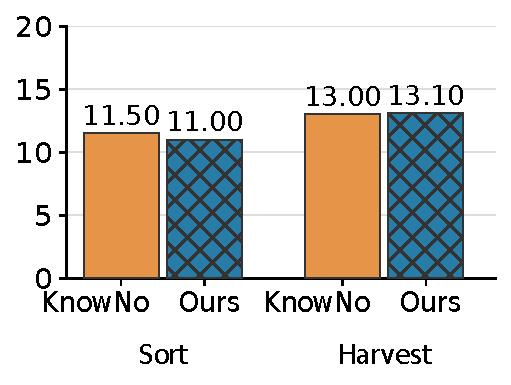
\includegraphics[width=\linewidth,height=.20\textheight,keepaspectratio]{figures/06_HUMAN_BASELINE/exp_human_plan_length.pdf}
\caption{Plan length (actions).}
\label{fig:human_human_plan_length}
\end{subfigure}
\par\smallskip
\begin{subfigure}[t]{0.247\textwidth}
\centering
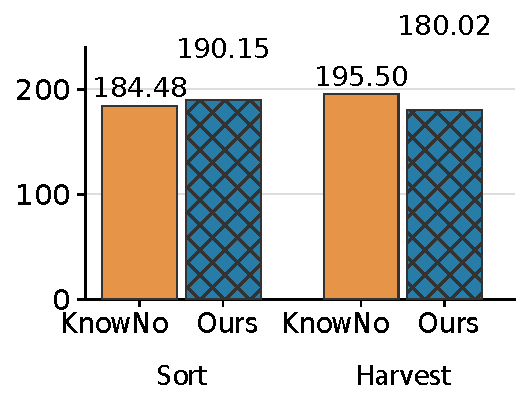
\includegraphics[width=\linewidth,height=.20\textheight,keepaspectratio]{figures/06_HUMAN_BASELINE/exp_human_total_time.pdf}
\caption{Total time (s).}
\label{fig:human_human_total_time}
\end{subfigure}%
\hspace{0.004\textwidth}%
\begin{subfigure}[t]{0.247\textwidth}
\centering
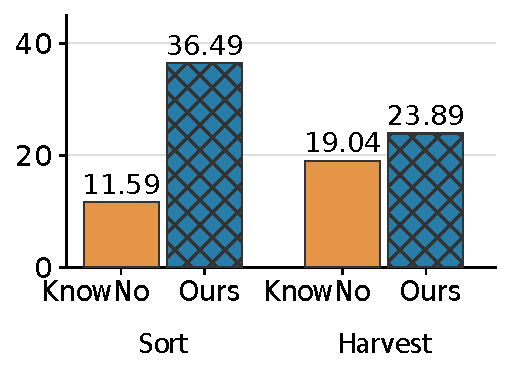
\includegraphics[width=\linewidth,height=.20\textheight,keepaspectratio]{figures/06_HUMAN_BASELINE/exp_human_interaction_time.pdf}
\caption{Interaction time (s).}
\label{fig:human_human_interaction_time}
\end{subfigure}%
\hspace{0.004\textwidth}%
\begin{subfigure}[t]{0.247\textwidth}
\centering
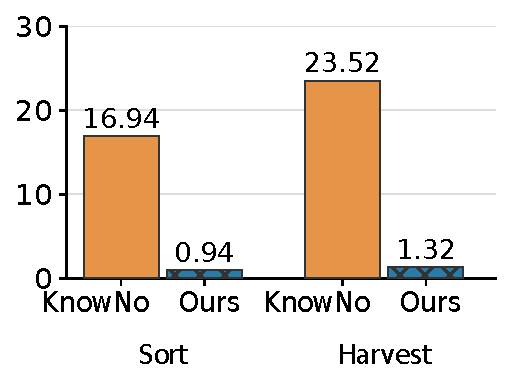
\includegraphics[width=\linewidth,height=.20\textheight,keepaspectratio]{figures/06_HUMAN_BASELINE/exp_human_planning_time.pdf}
\caption{Planning time (s).}
\label{fig:human_human_planning_time}
\end{subfigure}
\caption{Physical robot evaluation with human responses. (a)--(d) show success rate, query count, query probability, and plan length for WasteSorting and TomatoHarvesting. (e)--(g) show total time, interaction time, and planning time for both domains. An asterisk marks a metric based on a single successful trial, for which the sample standard deviation is undefined.}
\label{fig:human_results}
\end{figure*}








\noindent\textbf{Human}\label{exp:human_eval}.
We further examine whether the trends in task success and query behavior persist with human feedback. We recruited five participants (one man and four women), with a mean age of 26.4 years (SD = 5.68; range: 18--33 years). Eligibility required no visual recognition difficulties, including color vision deficiency.


We use the same robot platforms and task domains as in the VLM experiments. Participants receive instructions~\footnote{Appendix~\ref{appx:user} provides the detailed participant instructions and trial procedure.} about the task goals and available actions, then answer robot questions according to their own judgment through the tablet interface in Fig.~\ref{fig:human_tablet_interface}.


Each participant completes two trials with each method in each domain, for eight trials per participant and $10$ trials per method and domain. Trials are grouped by domain, and the domain and method orders vary across participants to reduce order effects (Table~\ref{tab:human_assignment}). Fig.~\ref{fig:human_results} shows the human results, and Table~\ref{tab:physical_robot_results} summarizes both the VLM and human results.

\begin{table}[!htbp]
\centering
\caption{Assigned order for the human evaluation. W.S. and T.H. denote WasteSorting and TomatoHarvesting. A denotes Ours and B denotes KnowNo. The method sequence applies to both domains for each participant.}
\label{tab:human_assignment}
\small
\setlength{\tabcolsep}{3pt}
\begin{tabular*}{\columnwidth}{@{\extracolsep{\fill}}cc@{}}
\toprule
Participant & Assigned order \\
\midrule
P01 & W.S. $\rightarrow$ T.H. : $A\rightarrow A\rightarrow B\rightarrow B$ \\
P02 & T.H. $\rightarrow$ W.S. : $A\rightarrow B\rightarrow A\rightarrow B$ \\
P03 & W.S. $\rightarrow$ T.H. : $B\rightarrow B\rightarrow A\rightarrow A$ \\
P04 & T.H. $\rightarrow$ W.S. : $B\rightarrow A\rightarrow B\rightarrow A$ \\
P05 & W.S. $\rightarrow$ T.H. : $A\rightarrow A\rightarrow B\rightarrow B$ \\
\bottomrule
\end{tabular*}
\end{table}


% Ours achieves a success rate of $90.00\%$ in WasteSorting and $100.00\%$ in TomatoHarvesting with human responses. KnowNo achieves $20.00\%$ and $30.00\%$ respectively. % 우리의 질이 방식이 oracle, vlm 뿐만 아니라 사람에게도 보여짐을 확인할 수 있다.

% Mean query counts are $7.11$ for Ours and $3.00$ for KnowNo in WasteSorting and $8.50$ and $3.67$ in TomatoHarvesting. 


% % vlm 과 비교
% Mean planning time is $0.94$ seconds for Ours and $16.94$ seconds for KnowNo in WasteSorting and $1.32$ and $23.52$ seconds in TomatoHarvesting. In WasteSorting, interaction time and total time are $36.49$ and $190.15$ seconds for Ours compared with $11.59$ and $184.48$ seconds for KnowNo. In TomatoHarvesting, the corresponding times are $23.89$ and $180.02$ seconds for Ours compared with $19.04$ and $195.50$ seconds for KnowNo.

% % 사람은 vlm과 달리 질문을 망설이기도 했다. 따라서 각 조건별 고민한 시간을 가져왔다.
% Including both successful and failed trials, the mean interaction time per query is $4.71$ seconds for Ours and $3.84$ seconds for KnowNo in WasteSorting and $2.73$ and $5.95$ seconds respectively in TomatoHarvesting. 

% % 특정 도메인에서는 또 질의 수는 우리가 더 많았는데, 전체 시간은 작았다. 
% KnowNo uses $57.81\%$ fewer queries than Ours in WasteSorting and $56.86\%$ fewer in TomatoHarvesting. However the lower query counts do not consistently reduce total time. Plan lengths are similar across methods, with $11.00$ physical actions for Ours and $11.50$ for KnowNo in WasteSorting and $13.10$ and $13.00$ respectively in TomatoHarvesting. Despite the additional queries, Ours requires $7.92\%$ less total time in TomatoHarvesting, while its total time is $3.08\%$ longer in WasteSorting.

Ours achieves a success rate of $90.00\%$ in WasteSorting and $100.00\%$ in TomatoHarvesting with human responses. KnowNo achieves $20.00\%$ and $30.00\%$ respectively. These results are consistent with the oracle and VLM comparisons and show that our method also achieves higher task success with human feedback. 
% Mean query counts are $7.11$ for Ours and $3.00$ for KnowNo in WasteSorting and $8.50$ and $3.67$ in TomatoHarvesting.
Consistent with the VLM experiments, Ours requires less planning time than KnowNo. Mean planning time is $0.94$ seconds for Ours and $16.94$ seconds for KnowNo in WasteSorting and $1.32$ and $23.52$ seconds in TomatoHarvesting. Participants also need time to inspect the displayed information and choose a response. We compute the mean interaction time per query by dividing total interaction time by the total number of queries across successful and failed trials. The values are $5.26$ seconds for Ours and $3.86$ seconds for KnowNo in WasteSorting and $2.81$ and $6.42$ seconds in TomatoHarvesting. One WasteSorting trial with Ours for P3 records $159.44$ seconds of interaction over nine queries, including one query lasting $77.00$ seconds. The experimenter observed that P3 hesitated when answering after consecutive task failures in the preceding trials. To examine the influence of P3's interaction times, we repeat the calculation after excluding all eight of P3's trials, covering both Ours and KnowNo in both domains. The mean interaction time per query is then $3.07$ seconds for Ours and $3.24$ seconds for KnowNo in WasteSorting and $2.64$ and $4.99$ seconds in TomatoHarvesting. % 이렇게 나온 이유를 작성해줘. 

% 성공·실패를 포함한 전체 interaction time을 전체 질의 수로 나눈 값이다. 시행별 평균을 다시 평균하지 않았다.
% WasteSorting은 Ours 378.7884초 / 72회 = 5.26초, KnowNo 111.9804초 / 29회 = 3.86초다.
% TomatoHarvesting은 Ours 238.9132초 / 85회 = 2.81초, KnowNo 218.3122초 / 34회 = 6.42초다.
% TomatoHarvesting의 KnowNo에서는 다음 행동과 선행 단계의 실행 여부를 함께 판단해야 했다. 인터뷰에서도 이러한 고민이 보고되어, 행동 선택에 시간이 더 들었을 가능성이 있다.
% WasteSorting의 Ours에는 약 77.00초가 걸린 개별 질의가 포함되어 평균을 높였다. 따라서 모든 조건에서 Ours의 질의당 시간이 짧게 나온 것은 아니다.
% 위 수치는 긴 응답도 제외하지 않은 전체 평균이다. 약 77.00초의 응답이 발생한 구체적 이유는 해당 질의의 진행 기록을 대조해 설명할 수 있다.
% 실험자 관찰: P3은 앞선 시행에서 실패를 연속으로 경험한 뒤 응답 선택을 망설였다.
% 사용자가 확인한 진행 순서는 실패-실패-실패(약 50초)-성공(약 150초) / 실패-실패-성공-성공이다.
% 위 약 50초·150초는 실험자가 설명한 진행 맥락의 시간이며, 로그의 누적 interaction time 159.4361초와 같은 측정값으로 취급하지 않는다.
% 따라서 긴 응답시간은 앞선 실패 경험 이후 나타난 망설임이라는 실험자 관찰과 함께 설명한다.


In successful TomatoHarvesting trials, interaction time is $23.89$ seconds for Ours compared with $19.04$ seconds for KnowNo. Total time is $180.02$ seconds for Ours compared with $195.50$ seconds for KnowNo, a reduction of $7.92\%$. In WasteSorting, total time is $190.15$ seconds for Ours compared with $184.48$ seconds for KnowNo, an increase of $3.08\%$. Thus fewer queries do not consistently reduce total task time.

\cp{Ours also achieves higher task success than KnowNo with human responses. These results suggest that query timing determines whether participants have an opportunity to correct robot decisions. Even if a participant notices an incorrect judgment, there may be no opportunity to correct it if the robot proceeds without a query. P01 reported that KnowNo proceeded without a query in situations where they wanted to intervene. Our method requests additional information if belief confidence is insufficient and incorporates human responses into subsequent planning.}






\noindent\textbf{Comparison across Feedback Sources}~\label{exp:response_comparison}. \cp{Fig.~\ref{fig:response_comparison} compares task success and query count across oracle, VLM, and human feedback. Ours achieves higher success rates and uses more queries than KnowNo in both domains across all three feedback sources. However the magnitude of the success advantage depends on the domain and feedback source. In WasteSorting, Ours maintains success rates of $100.00\%$, $92.50\%$, and $100.00\%$ with oracle, VLM, and human feedback respectively. In TomatoHarvesting, success decreases from $98.00\%$ with oracle feedback to $92.50\%$ with VLM feedback and $50.00\%$ with human feedback. The success advantage over KnowNo also narrows from $55.00$ percentage points with oracle feedback to $16.67$ percentage points with human feedback in TomatoHarvesting. Thus the relative advantage of Ours persists, but high success does not persist equally across domains and feedback sources.

Query counts also show differences across feedback sources. In TomatoHarvesting, Ours uses $9.16$, $8.51$, and $9.67$ queries with oracle, VLM, and human feedback respectively. KnowNo uses $2.45$, $7.20$, and $4.00$ queries. The query count of KnowNo increases substantially with VLM feedback, while the query count of Ours remains similar across feedback sources despite the lower success with human feedback. Therefore similar query counts do not imply similar task outcomes, and the number of queries alone does not explain the differences across feedback sources. These differences motivate the subsequent human interview analysis. We examine how participants interpret robot questions and what reasoning participants need to choose a response, with particular attention to question clarity and response effort.}



\begin{figure*}[!tp]
\centering
\begin{subfigure}[t]{0.495\textwidth}
\centering
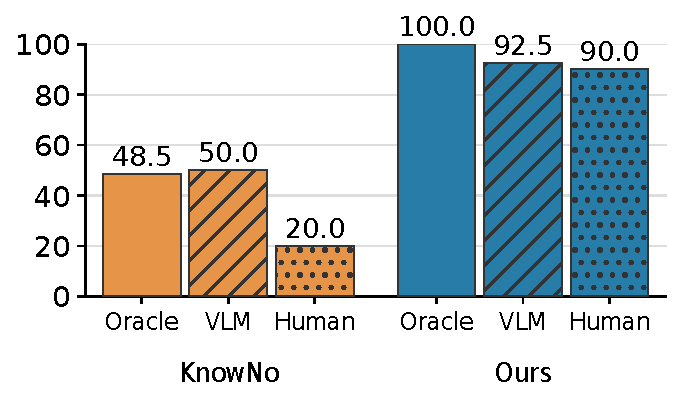
\includegraphics[width=\linewidth,height=.20\textheight,keepaspectratio]{figures/07_RESPONSE_COMPARISON/exp_response_waste_success.pdf}
\caption{W.S. Success rate (\%).}
\label{fig:response_response_waste_success}
\end{subfigure}
\hfill
\begin{subfigure}[t]{0.495\textwidth}
\centering
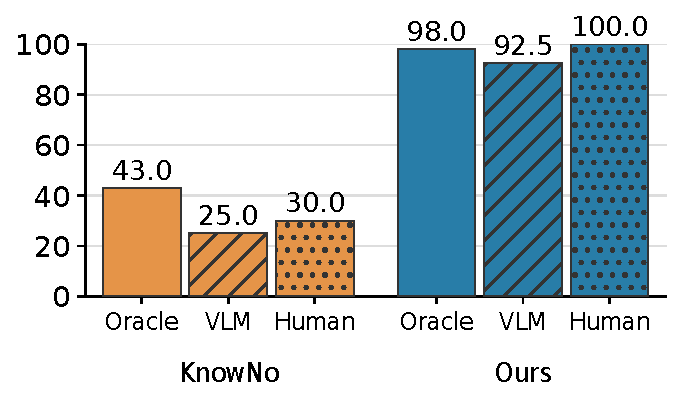
\includegraphics[width=\linewidth,height=.20\textheight,keepaspectratio]{figures/07_RESPONSE_COMPARISON/exp_response_tomato_success.pdf}
\caption{T.H. Success rate (\%).}
\label{fig:response_response_tomato_success}
\end{subfigure}
\par\medskip
\begin{subfigure}[t]{0.495\textwidth}
\centering
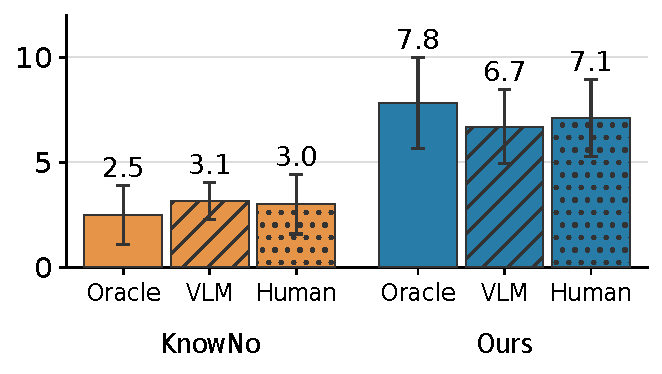
\includegraphics[width=\linewidth,height=.20\textheight,keepaspectratio]{figures/07_RESPONSE_COMPARISON/exp_response_waste_queries.pdf}
\caption{W.S. Query count.}
\label{fig:response_response_waste_queries}
\end{subfigure}
\hfill
\begin{subfigure}[t]{0.495\textwidth}
\centering
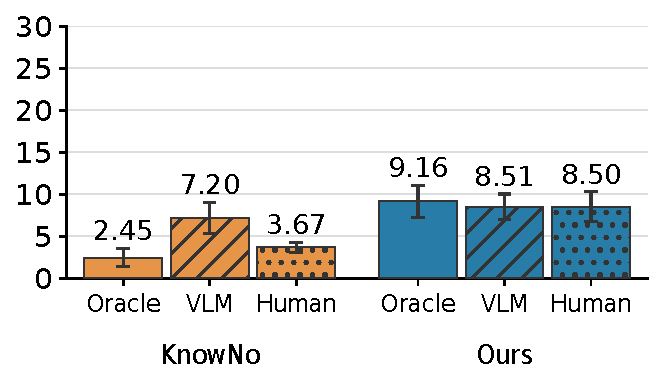
\includegraphics[width=\linewidth,height=.20\textheight,keepaspectratio]{figures/07_RESPONSE_COMPARISON/exp_response_tomato_queries.pdf}
\caption{T.H. Query count.}
\label{fig:response_response_tomato_queries}
\end{subfigure}
\caption{Comparison across oracle, VLM, and human responses. (a)--(b) show success rates for WasteSorting and TomatoHarvesting, respectively. (c)--(d) show query counts for the same domains in the same order. Oracle trials use simulation, while VLM and human trials use physical robots.}\label{fig:response_comparison}
\end{figure*}





\subsubsection{Ablation Study}~\label{exp:when_what_random}\label{exp:policy_ablation}

We conduct an ablation study to assess the contributions of query timing and query selection to task success and query efficiency. We compare seven configurations with oracle feedback in simulation. For concise reference, we use \textbf{W} to label query timing variants and \textbf{Q} to label query selection variants. With entropy gain selection fixed, we compare random (W1), conformal prediction (W2), and reward-based (W3) timing. With confidence timing fixed, we compare random (Q1) and reward-based (Q2) selection. Fully-Random randomizes both query timing and query selection, while Ours combines confidence timing with entropy gain selection. Table~\ref{tab:query_strategy_matrix} summarizes these configurations. Each configuration has $200$ trials per domain. Table~\ref{tab:policy_ablation} and Fig.~\ref{fig:policy_ablation_results} present the results. Appendix~\ref{appx:ablation_configs} provides the query policy configurations.

\begin{figure*}[!tp]
\centering
\begin{subfigure}[t]{0.495\textwidth}
\centering
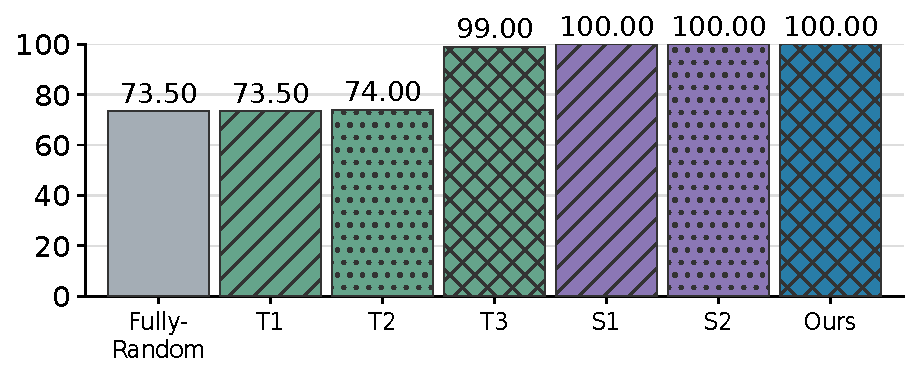
\includegraphics[width=\linewidth,height=.20\textheight,keepaspectratio]{figures/08_ABLATION/exp_ablation_waste_success.pdf}
\caption{W.S. Success rate (\%).}
\label{fig:ablation_ablation_waste_success}
\end{subfigure}
\hfill
\begin{subfigure}[t]{0.495\textwidth}
\centering
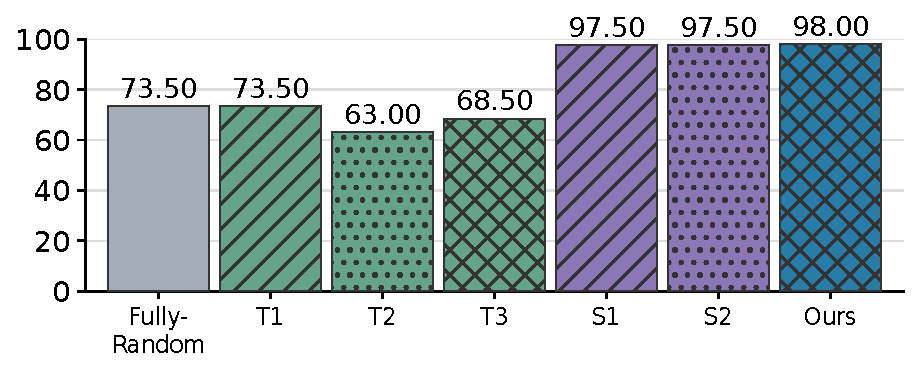
\includegraphics[width=\linewidth,height=.20\textheight,keepaspectratio]{figures/08_ABLATION/exp_ablation_tomato_success.pdf}
\caption{T.H. Success rate (\%).}
\label{fig:ablation_ablation_tomato_success}
\end{subfigure}
\par\medskip
\begin{subfigure}[t]{0.495\textwidth}
\centering
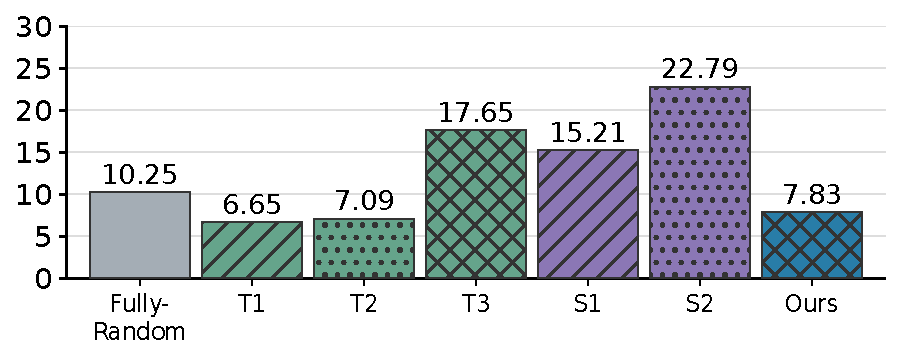
\includegraphics[width=\linewidth,height=.20\textheight,keepaspectratio]{figures/08_ABLATION/exp_ablation_waste_queries.pdf}
\caption{W.S. Query count.}
\label{fig:ablation_ablation_waste_queries}
\end{subfigure}
\hfill
\begin{subfigure}[t]{0.495\textwidth}
\centering
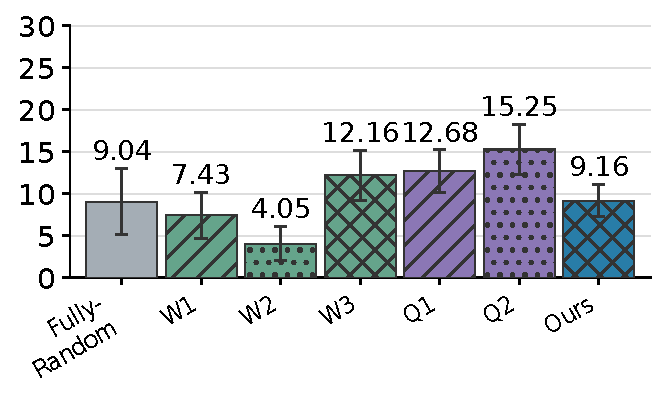
\includegraphics[width=\linewidth,height=.20\textheight,keepaspectratio]{figures/08_ABLATION/exp_ablation_tomato_queries.pdf}
\caption{T.H. Query count.}
\label{fig:ablation_ablation_tomato_queries}
\end{subfigure}
\caption{Query timing and selection ablation. (a)--(b) show success rates for WasteSorting and TomatoHarvesting, respectively. (c)--(d) show query counts for the same domains in the same order. W1--W3 vary query timing, while Q1--Q2 vary query selection. The results suggest that timing based on belief confidence supports task success, while selection by expected entropy reduction reduces the number of queries required.}
\label{fig:policy_ablation_results}
\end{figure*}


\begin{table*}[t]
\centering
\caption{Query policy ablation. W1--W3 compare timing criteria and Q1--Q2 compare selection criteria.}
\label{tab:policy_ablation}
\label{tab:when_what_random}
\small
\setlength{\tabcolsep}{4pt}
\begin{tabular}{lllcccc}
\toprule
 & & & \multicolumn{2}{c}{WasteSorting} & \multicolumn{2}{c}{TomatoHarvesting} \\
\cmidrule(lr){4-5}\cmidrule(lr){6-7}
Condition & Timing & Selection & Success (\%) & Queries & Success (\%) & Queries \\
\midrule
Fully-Random & Random & Random & 73.50 & $10.25 \pm 6.11$ & 73.50 & $9.04 \pm 3.94$ \\
W1 & Random & Entropy Gain & 73.50 & $6.65 \pm 3.29$ & 73.50 & $7.43 \pm 2.72$ \\
W2 & Conformal Prediction & Entropy Gain & 74.00 & $7.09 \pm 2.58$ & 63.00 & $4.05 \pm 2.04$ \\
W3 & Reward & Entropy Gain & 99.00 & $17.65 \pm 2.89$ & 68.50 & $12.16 \pm 3.00$ \\
Q1 & Confidence & Random & 100.00 & $15.21 \pm 3.53$ & 97.50 & $12.68 \pm 2.53$ \\
Q2 & Confidence & Reward & 100.00 & $22.79 \pm 6.26$ & 97.50 & $15.25 \pm 2.95$ \\
Ours & Confidence & Entropy Gain & 100.00 & $7.83 \pm 2.16$ & 98.00 & $9.16 \pm 1.90$ \\
\bottomrule
\end{tabular}
\end{table*}

The timing comparison evaluates Fully-Random, W1--W3, and Ours. In WasteSorting, Fully-Random and W1 achieve $73.50\%$ success, and W2 achieves $74.00\%$. W3 achieves $99.00\%$ compared with $100.00\%$ for Ours, but requires $17.65$ queries compared with $7.83$. Fully-Random, W1, and W2 use $10.25$, $6.65$, and $7.09$ queries respectively. In TomatoHarvesting, Fully-Random and W1 achieve $73.50\%$ success, while W2 and W3 achieve $63.00\%$ and $68.50\%$ compared with $98.00\%$ for Ours. Mean query counts are $9.04$ for Fully-Random, $7.43$ for W1, $4.05$ for W2, $12.16$ for W3, and $9.16$ for Ours.

These results show that task success depends on the query trigger as well as query selection. W1 replaces random selection in Fully-Random with entropy gain and reduces query count without improving success. Random timing can miss necessary verification because the trigger does not depend on current state uncertainty. W2 can also end queries after the action prediction set narrows to one candidate, even if the state facts required to execute the candidate action remain uncertain. W3 uses expected task reward to determine whether to initiate queries, then selects queries by entropy gain and repeats verification until confidence reaches $\tau$. In WasteSorting, object category verification directly informs the correct bin choice and task reward, so repeated verification may support the high success rate of $99.00\%$. However W3 requires $125.43\%$ more queries than Ours. In TomatoHarvesting, W3 uses $32.71\%$ more queries than Ours, but the success rate of W3 is $29.50$ percentage points lower. Therefore reward-based timing can request more queries overall and still fail to verify necessary state information at the appropriate time. Thus Ours uses current state confidence as the query trigger and achieves the highest success in both domains with fewer queries than reward-based timing.

With confidence-based query timing fixed, different query selection strategies maintain high success rates but require different numbers of queries. The query selection comparison evaluates Fully-Random, Q1, Q2, and Ours. Fully-Random achieves $73.50\%$ success in both domains with $10.25$ queries in WasteSorting and $9.04$ in TomatoHarvesting. Q1 retains random selection but uses confidence timing, and success increases to $100.00\%$ and $97.50\%$ respectively. With confidence timing fixed, Q1, Q2, and Ours all achieve $100.00\%$ success in WasteSorting. Mean query counts are $15.21$ for Q1, $22.79$ for Q2, and $7.83$ for Ours. In TomatoHarvesting, Q1 and Q2 achieve $97.50\%$ success compared with $98.00\%$ for Ours. Mean query counts are $12.68$ for Q1, $15.25$ for Q2, and $9.16$ for Ours.

Confidence timing maintains $100.00\%$ success in WasteSorting and at least $97.50\%$ in TomatoHarvesting across all three query selection strategies. Under confidence timing, query selection primarily affects the number of queries needed to reach the required confidence. Random selection does not prioritize facts by their expected reduction in state uncertainty. Reward-based selection evaluates expected task reward without directly measuring the information provided by a query response. Entropy gain selects facts according to the expected reduction in state uncertainty, so the selection criterion matches the confidence requirement that ends a query episode. Relative to Q1 and Q2, Ours reduces query count by $48.54\%$ and $65.64\%$ in WasteSorting and by $27.72\%$ and $39.92\%$ in TomatoHarvesting. Thus our query selection method reduces the number of queries required under confidence timing without reducing task success.

These results support the main contribution of our method through the distinct roles of query timing and query selection. Query timing determines whether the robot requests additional information before it executes actions under state uncertainty. Confidence timing achieves high success with random, reward-based, and entropy gain selection, while entropy gain under random timing reduces query count without improving success over Fully-Random. Once confidence timing establishes a high success level, entropy gain reduces the number of queries needed to reach the required confidence. Therefore our method combines a timing criterion that supports task success with a selection criterion that reduces query count at that success level.

\subsubsection{Threshold Experiments}~\label{exp:sys_threshold}

After the ablation comparison, we examine how the confidence threshold controls task success and query count. We vary $\tau$ from $0.0$ to $1.0$ in increments of $0.1$ with entropy gain selection fixed and correct oracle responses in simulation. Each threshold has $200$ trials per domain. Table~\ref{tab:threshold_results} and Fig.~\ref{fig:threshold_results} present the results. The results at $\tau=0.8$ use the same Ours trials as the baseline and ablation comparisons, as specified in Appendix~\ref{appx:oracle_reference}.

\begin{figure*}[!tp]
\centering
\begin{subfigure}[t]{0.49\textwidth}
\centering
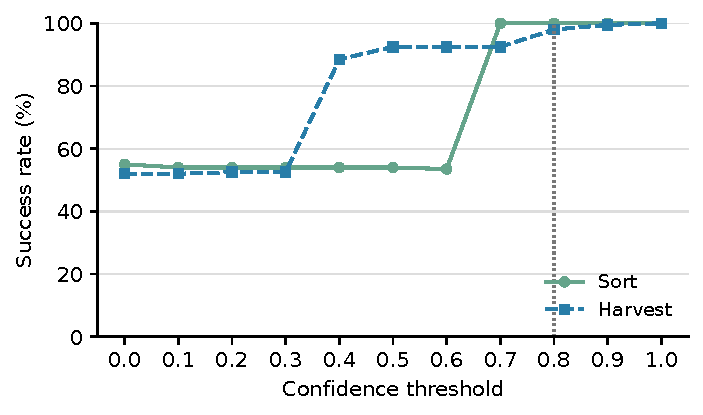
\includegraphics[width=\linewidth]{figures/09_THRESHOLD/exp_threshold_success.pdf}
\caption{Task success.}
\label{fig:threshold_success}
\end{subfigure}
\hfill
\begin{subfigure}[t]{0.49\textwidth}
\centering
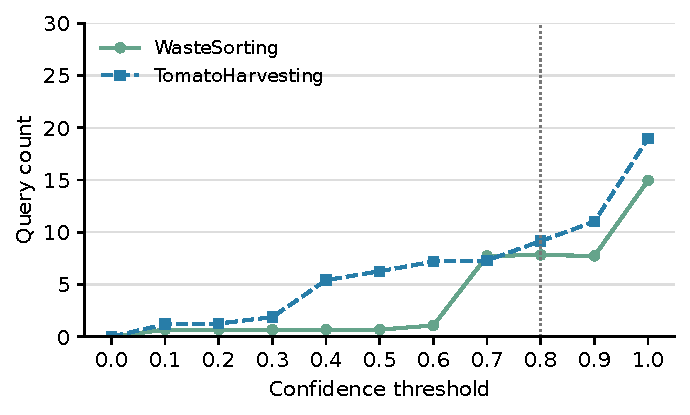
\includegraphics[width=\linewidth]{figures/09_THRESHOLD/exp_threshold_queries.pdf}
\caption{Mean query count.}
\label{fig:threshold_queries}
\end{subfigure}
\caption{Effect of the confidence threshold on task success and query count. (a) shows success rates and (b) shows mean query counts for WasteSorting and TomatoHarvesting. The dotted line marks the default threshold of $\tau=0.8$. Compared with $\tau=0.8$, $\tau=1.0$ nearly doubles query count with little or no improvement in task success.}
\label{fig:threshold_results}
\end{figure*}


\begin{table}[t]
\centering
\caption{Task success and query count across confidence thresholds.}
\label{tab:threshold_results}
\small
\setlength{\tabcolsep}{1pt}
\begin{tabular*}{\columnwidth}{@{\extracolsep{\fill}}ccccc@{}}
\toprule
 & \multicolumn{2}{c}{WasteSorting} & \multicolumn{2}{c}{TomatoHarvesting} \\
\cmidrule(lr){2-3}\cmidrule(lr){4-5}
$\tau$ & Success (\%) & Queries & Success (\%) & Queries \\
\midrule
0.0 & 55.00 & $0.00 \pm 0.00$ & 52.00 & $0.00 \pm 0.00$ \\
0.1 & 54.00 & $0.69 \pm 0.84$ & 52.00 & $1.21 \pm 1.43$ \\
0.2 & 54.00 & $0.69 \pm 0.84$ & 52.50 & $1.27 \pm 1.42$ \\
0.3 & 54.00 & $0.69 \pm 0.84$ & 52.50 & $1.89 \pm 1.83$ \\
0.4 & 54.00 & $0.69 \pm 0.84$ & 88.50 & $5.42 \pm 2.30$ \\
0.5 & 54.00 & $0.69 \pm 0.84$ & 92.50 & $6.27 \pm 2.07$ \\
0.6 & 53.50 & $1.08 \pm 0.97$ & 92.50 & $7.20 \pm 1.99$ \\
0.7 & 100.00 & $7.74 \pm 2.25$ & 92.50 & $7.30 \pm 2.04$ \\
0.8 & 100.00 & $7.83 \pm 2.16$ & 98.00 & $9.16 \pm 1.90$ \\
0.9 & 100.00 & $7.74 \pm 2.25$ & 99.50 & $11.02 \pm 1.52$ \\
1.0 & 100.00 & $14.97 \pm 2.02$ & 100.00 & $19.00 \pm 1.43$ \\
\bottomrule
\end{tabular*}
\end{table}


In WasteSorting, success improves sharply at $\tau=0.7$ and remains constant at higher thresholds. With $\tau=0.0$, the robot makes no queries and achieves $55.00\%$ success. Thresholds from $0.1$ to $0.6$ yield success rates between $53.50\%$ and $54.00\%$ with at most $1.08$ queries on average. At $\tau=0.7$, success reaches $100.00\%$ with $7.74$ queries. Success remains $100.00\%$ over $\tau=0.7$--$0.9$, and query count stays between $7.74$ and $7.83$. However $\tau=1.0$ requires $14.97$ queries without further success improvement. The additional queries confirm that the strictest confidence requirement can increase interaction frequency after task success reaches its maximum.

In TomatoHarvesting, higher thresholds improve success over a wider range. Success is $52.00\%$ without queries at $\tau=0.0$ and remains at most $52.50\%$ through $\tau=0.3$. At $\tau=0.4$, success increases to $88.50\%$ with $5.42$ queries. Success reaches $92.50\%$ over $\tau=0.5$--$0.7$ and $98.00\%$ at $\tau=0.8$ with $9.16$ queries. Raising $\tau$ to $0.9$ increases success to $99.50\%$ with $11.02$ queries. At $\tau=1.0$, success reaches $100.00\%$ with $19.00$ queries. Therefore the increase from $0.9$ to $1.0$ adds $7.98$ queries for only $0.50$ percentage points of additional success.

The two domains require different confidence levels to reach high success, but both show limited gains from the strictest threshold. Relative to $\tau=0.8$, $\tau=1.0$ increases query count by $91.19\%$ in WasteSorting and $107.30\%$ in TomatoHarvesting. Success improves by $0.00$ and $2.00$ percentage points respectively. We use $\tau=0.8$ as a common threshold because it achieves $100.00\%$ and $98.00\%$ success in the two domains with substantially fewer queries than $\tau=1.0$. Thus the threshold controls the amount of state verification, and the highest confidence requirement does not provide a proportional improvement in task success.

\subsubsection{Interviews}\label{exp:interviews}
\cp{The interviews examined how participants understood and answered queries after they experienced both methods in WasteSorting and TomatoHarvesting. We focused on the judgments required to answer questions, perceived effort across the task, and difficulties with the displayed information.}

\cp{Participants described different judgments required by the two methods. P01 explained that Ours required only an assessment of the current situation, without the need to anticipate the next action. For KnowNo, P01 considered which actions had to occur first and whether a proposed action could be executed at that point. P01 also found it unclear whether an action choice implied that the robot would perform the necessary preceding actions. P02 described the questions from Ours as simpler and reported less need to think before answering.}

\cp{Perceived effort across the entire task differed between participants. P01 found Ours more laborious because questions occurred more frequently, but reported greater satisfaction because the judgments were clearer and execution followed the intended course. P02 described Ours as less laborious and felt that the robot made more of the decisions. Thus, easier individual judgments did not imply uniformly lower effort across the task.}

\cp{Participants also described difficulties with the information provided for their judgments. P01 reported that a mismatch between object identifiers in the question and the image made the referenced tomato unclear. P02 reported that occlusion by the gripper made it difficult to judge the condition of a tomato from the camera view. P01 also requested a way to revise an earlier answer before the robot executed an action.}

\subsubsection{Discussion}\label{exp:discussion}

Results with oracle, VLM, and human responses support the effectiveness of our method. Query timing and query selection serve complementary roles. The confidence threshold determines when to query based on state uncertainty, while expected entropy reduction determines which information to request. The ablation experiments highlight the importance of both decisions. Effective query selection can reduce the number of queries, but reliable execution also depends on requesting information when state is uncertain.

The objective is to obtain sufficient state information for successful execution while limiting the number of queries. A stricter confidence requirement can increase the number of queries without a corresponding improvement in task success. Thus, reducing uncertainty beyond what is needed for successful execution may introduce unnecessary interaction. These findings suggest that effective querying requires balancing the information needed for reliable execution against the cost of obtaining it.

Beyond task performance, the interviews also provide indirect insight into \textit{how} to query people. Participants described our state questions as easier to judge and reported less need to think before answering than with KnowNo. This feedback supports the use of the proposed state questions for human assistance. However, \textit{how} also includes interaction modalities and UI design, which can affect usability and cognitive workload. We did not compare voice interfaces or alternative UI designs, and their effects on human interaction remain future work.


% % Keep the experimental figures and tables before the conclusion.
% \clearpage

\section{Conclusion and Future Work}
We presented a method that uses state uncertainty to determine when and what to query during robot task execution. Belief confidence determines query timing, and expected entropy reduction guides the selection of state facts. Experiments in WasteSorting and TomatoHarvesting show that query timing supports task success, while query selection reduces the number of required queries. Future work will examine multi-modal interfaces and UI design for human interaction.

\bmhead{Acknowledgements}
This research was supported in part by the National Research Foundation of Korea (NRF) grant funded by the Korea government (MSIT)(No. RS-2024-00461583) and the National Research Foundation of Korea (NRF) grant funded by the Korea government (MSIT) (No. RS-2024-00411007).

\bmhead{Ethics approval and consent}
This study was approved by the Institutional Review Board of Sogang University (Approval No. SGUIRB-A-2501-04-2). The study was conducted in accordance with the ethical standards of the institution. Informed consent was obtained from all participants before participation.

\bibliography{ref}

\begin{appendices}
\onecolumn
\section{Detailed Experimental Settings}~\label{appx:settings}

This appendix specifies the planner settings, query policies, domain models, and reporting conventions for Sec.~\ref{exp:setup}. The oracle experiments use simulated execution with correct responses. The VLM and human evaluations use physical robot execution. We aggregate trials within each domain for all reported comparisons.

\subsection{Planner and Evaluation Parameters}~\label{appx:planner_params}
Table~\ref{tab:app_planner_params} lists the default POMCP parameters for Ours. The oracle trial limit is $50$ physical actions, and the physical trial limit is $20$. Queries do not consume physical steps for Ours. POMCP-Q uses a limit of $50$ total decisions that includes queries and physical actions. \cp{Seven WasteSorting trials and $13$ TomatoHarvesting trials terminate at this limit.} The reward-based configurations use the discount factors specified below.

\begin{table}[!htbp]
\centering
\caption{Planner and evaluation parameters used by Ours.}
\label{tab:app_planner_params}
\small
\begin{tabular}{lc}
\toprule
\textbf{Parameter} & \textbf{Value} \\
\midrule
POMCP simulations per planning step & $100$ \\
Maximum simulation depth & $20$ \\
Discount factor $\gamma$ & $0.2$ \\
UCB exploration constant $c$ & $1.0$ \\
Oracle physical action limit & $50$ \\
Physical action limit & $20$ \\
Default confidence threshold $\tau$ & $0.8$ \\
Discount cutoff $\epsilon$ & $0.005$ \\
Oracle frontier capacity & $8{,}000$ \\
Oracle search-node particle capacity & $8{,}000$ \\
Oracle transition sampling budget & $250$ \\
Oracle initial configurations per domain & $5$ \\
Trials per initial configuration and condition & $40$ \\
Oracle trials per domain and condition & $200$ \\
\bottomrule
\end{tabular}
\end{table}

\cp{With $\gamma=0.2$ and $\epsilon=0.005$, the discount cutoff stops search at depth $4$ before the nominal maximum of $20$.}

\subsection{Baseline Configurations}~\label{appx:baseline_configs}
The oracle baseline comparison evaluates KnowNo, IntroPlan, and POMCP-Q against Ours. The physical experiments compare KnowNo and Ours. Appendix~\ref{appx:baseline_algorithms} provides separate procedures for the three baselines. KnowNo and IntroPlan use GPT-4o for action generation and candidate scoring. This planning model is separate from Gemma 4 31B IT, which provides external feedback in the VLM experiments.

The \cp{recorded} action generation temperature is $0.3$, and the candidate score temperature is $5.0$. KnowNo uses calibration thresholds $\hat{q}=0.845165$ for WasteSorting and $\hat{q}=\cp{0.8404}$ for TomatoHarvesting in the oracle comparison. The physical VLM logs \cp{use $0.845165$ and $0.901119$ respectively}, except for one WasteSorting trial with $\hat{q}=0.8704$. \cp{The oracle TomatoHarvesting KnowNo batch does not record the generation temperature.} IntroPlan retrieves three examples and uses calibration thresholds $0.980493$ and $0.985552$ for the two domains in the same order. POMCP-Q uses the \cp{recorded domain-specific configuration}. The discount factor is $0.9$ for WasteSorting and $0.5$ for TomatoHarvesting. Query cost is zero, the failure penalty is $10$, assumed response accuracy is $1.0$, and the planner uses $100$ simulations per decision.

% Source: experiments_logs/query_action_tuning/20260921_130229_529697/analysis/
% report.md, selected_config.json, and 01_processed/episodes.csv (1,200 trials).
A preliminary POMCP-Q sweep tested $\gamma\in\{0.2,0.5,0.8,0.95\}$ and query costs $\{0,0.5,1\}$, with ten trials per scene in each domain for every pair. The selection criterion was the highest pooled task success rate: $\gamma=0.5$ with zero query cost achieved $66/100$ successes. This supports the zero-cost setting and the TomatoHarvesting discount factor used in the reported configurations.
% TODO(author): Explain the later WasteSorting choice gamma=0.9. It is verified
% in the final execution logs but is absent from the above sweep; the sweep
% winner was gamma=0.5 for the pooled objective, not a domain-specific optimum.

\cp{Tables~\ref{tab:app_baseline_params_waste} and~\ref{tab:app_baseline_params_tomato} summarize the baseline parameters for each domain.}

\begin{table*}[!htbp]
\centering
\caption{Baseline parameters for WasteSorting.}
\label{tab:app_baseline_params_waste}
\small
\setlength{\tabcolsep}{5pt}
\renewcommand{\arraystretch}{1.12}
\begin{tabular*}{\textwidth}{@{\extracolsep{\fill}}lcccc@{}}
\toprule
Parameter & Ours & KnowNo & IntroPlan & POMCP-Q \\
\midrule
Action generation/scoring model & --- & GPT-4o & GPT-4o & --- \\
Calibration threshold $\hat{q}$ (oracle) & --- & $0.845165$ & $0.980493$ & --- \\
Action generation temperature (oracle) & --- & $0.3$ & $0.3$ & --- \\
Candidate score temperature & --- & $5.0$ & $5.0$ & --- \\
Retrieved examples & --- & --- & $3$ & --- \\
Discount factor $\gamma$ & $0.2$ & --- & --- & $0.9$ \\
POMCP simulations per decision & $100$ & --- & --- & $100$ \\
Confidence threshold $\tau$ & $0.8$ & --- & --- & --- \\
Query evaluation cost & --- & --- & --- & $0$ \\
Failure penalty & --- & --- & --- & $10$ \\
Assumed response accuracy & --- & --- & --- & $1.0$ \\
Oracle trial limit & $50$ actions & $50$ actions & $50$ actions & $50$ decisions \\
KnowNo calibration $\hat{q}$ (physical VLM) & --- & $0.845165$ & --- & --- \\
\bottomrule
\end{tabular*}
\par\smallskip
\begin{minipage}{\textwidth}
\footnotesize A dash denotes a setting that does not apply to the listed method or query evaluator. Oracle settings are shown unless the row specifies physical VLM execution. POMCP-Q counts both queries and physical actions toward its decision limit. Common planner settings appear in Table~\ref{tab:app_planner_params}.
\end{minipage}
\end{table*}

\begin{table*}[!htbp]
\centering
\caption{Baseline parameters for TomatoHarvesting.}
\label{tab:app_baseline_params_tomato}
\small
\setlength{\tabcolsep}{5pt}
\renewcommand{\arraystretch}{1.12}
\begin{tabular*}{\textwidth}{@{\extracolsep{\fill}}lcccc@{}}
\toprule
Parameter & Ours & KnowNo & IntroPlan & POMCP-Q \\
\midrule
Action generation/scoring model & --- & GPT-4o & GPT-4o & --- \\
Calibration threshold $\hat{q}$ (oracle) & --- & $0.8404$ & $0.985552$ & --- \\
Action generation temperature (oracle) & --- & NR & $0.3$ & --- \\
Candidate score temperature & --- & $5.0$ & $5.0$ & --- \\
Retrieved examples & --- & --- & $3$ & --- \\
Discount factor $\gamma$ & $0.2$ & --- & --- & $0.5$ \\
POMCP simulations per decision & $100$ & --- & --- & $100$ \\
Confidence threshold $\tau$ & $0.8$ & --- & --- & --- \\
Query evaluation cost & --- & --- & --- & $0$ \\
Failure penalty & --- & --- & --- & $10$ \\
Assumed response accuracy & --- & --- & --- & $1.0$ \\
Oracle trial limit & $50$ actions & $50$ actions & $50$ actions & $50$ decisions \\
KnowNo calibration $\hat{q}$ (physical VLM) & --- & $0.901119$ & --- & --- \\
\bottomrule
\end{tabular*}
\par\smallskip
\begin{minipage}{\textwidth}
\footnotesize A dash denotes a setting that does not apply to the listed method or query evaluator. Oracle settings are shown unless the row specifies physical VLM execution. POMCP-Q counts both queries and physical actions toward its decision limit. Common planner settings appear in Table~\ref{tab:app_planner_params}. NR denotes an action generation temperature not recorded in the oracle KnowNo batch.
\end{minipage}
\end{table*}

\subsection{Ablation Configurations}~\label{appx:ablation_configs}
We distinguish the criterion for entering a query episode, the rule for selecting each fact, and the criterion for ending the episode. These decisions follow the belief update from a physical observation and precede the next physical action.

\noindent\textbf{Entry.} Fully-Random and W1 enter with probability $0.4$ per physical step. Ours, Q1, and Q2 enter when belief confidence is below $\tau=0.8$. W2 enters unless the conformal action prediction set contains exactly one concrete action; an empty set or a set containing the fallback option also triggers verification. W3 enters when the highest query-action value exceeds the highest applicable physical-action value.

\noindent\textbf{Selection.} Fully-Random and Q1 sample uniformly from facts that distinguish the remaining state hypotheses. Ours and W1--W3 select the fact with the largest expected entropy reduction, recomputed after each response. Thus neither W2's conformal set nor W3's highest-valued query specifies the fact actually asked. Q2 instead selects the highest-valued query fact and recomputes query values after each response; it does not compare them with physical-action values to cancel a query.

% The 396 valid archived W2 policy traces, not the current query_episode.py,
% verify repeated CP decisions. W3 uses the 20261005_204332_446690 rerun;
% Q2 uses the 20261005_190346_519071 batch. See asset/BRL_oracle_exp_v2/
% 02_when_what_policy_ablation/00_raw/ and EXPERIMENT_SETTINGS.md.
\noindent\textbf{Continuation and termination.} After entry, Fully-Random, W1, W3, Q1, Q2, and Ours continue until confidence reaches $\tau$ or no differentiating fact remains. W3 evaluates reward-based timing only on entry and has no one-question limit in the reported rerun. In contrast, the archived W2 batch used for the reported results reevaluates the conformal criterion after each fact response and stops when the set becomes a singleton concrete action or no differentiating fact remains. W2 can therefore stop below $\tau$; its continuation criterion differs from confidence-based verification. A failure to reduce the represented hypotheses also ends an episode in the policy runner.

W2 uses calibration thresholds $0.8704$ for WasteSorting and $0.8404$ for TomatoHarvesting, with score temperature $5.0$. Four unparseable outputs count as failures in the success rate and contribute no successful-trial cost measurements. Both reward-based variants use zero query cost, a failure penalty of $10$, and assumed response accuracy $1.0$. They reuse the domain-specific discount factors of POMCP-Q, $0.9$ for WasteSorting and $0.5$ for TomatoHarvesting, for both query evaluation and physical action planning. The query evaluator uses at least $100$ simulations and increases the budget to the number of root candidates plus one if necessary. The remaining configurations use $\gamma=0.2$. Consequently, comparisons with W3 and Q2 also change the discount factor, and the W2 comparison changes the continuation rule in addition to the entry criterion.

\cp{Tables~\ref{tab:app_ablation_params_waste} and~\ref{tab:app_ablation_params_tomato} summarize the ablation parameters for each domain.}

\begin{table*}[!htbp]
\centering
\caption{Ablation parameters for WasteSorting.}
\label{tab:app_ablation_params_waste}
\small
\setlength{\tabcolsep}{4pt}
\renewcommand{\arraystretch}{1.12}
\begin{tabular*}{\textwidth}{@{\extracolsep{\fill}}lccccccc@{}}
\toprule
Parameter & FR & W1 & W2 & W3 & Q1 & Q2 & Ours \\
\midrule
Query timing & Random & Random & CP & Reward & Confidence & Confidence & Confidence \\
Query selection & Random & Entropy & Entropy & Entropy & Random & Reward & Entropy \\
Random trigger probability & $0.4$ & $0.4$ & --- & --- & --- & --- & --- \\
Configured threshold $\tau$ & $0.8$ & $0.8$ & $0.8$ & $0.8$ & $0.8$ & $0.8$ & $0.8$ \\
Discount factor $\gamma$ & $0.2$ & $0.2$ & $0.2$ & $0.9$ & $0.2$ & $0.9$ & $0.2$ \\
POMCP simulations & $100$ & $100$ & $100$ & $100$ & $100$ & $100$ & $100$ \\
Calibration threshold $\hat{q}$ & --- & --- & $0.8704$ & --- & --- & --- & --- \\
Candidate score temperature & --- & --- & $5.0$ & --- & --- & --- & --- \\
Query evaluation cost & --- & --- & --- & $0$ & --- & $0$ & --- \\
Failure penalty & --- & --- & --- & $10$ & --- & $10$ & --- \\
Assumed response accuracy & --- & --- & --- & $1.0$ & --- & $1.0$ & --- \\
Query evaluation simulations & --- & --- & --- & $\geq 100$ & --- & $\geq 100$ & --- \\
\bottomrule
\end{tabular*}
\par\smallskip
\begin{minipage}{\textwidth}
\footnotesize FR denotes Fully-Random, and CP denotes conformal prediction. Entropy denotes selection by expected entropy gain. A dash denotes a setting that does not apply to the listed query policy. W2 uses the conformal prediction set to initiate and continue verification. The other configurations use confidence to continue verification after a trigger. All configurations use oracle feedback, a limit of $50$ physical actions, and $200$ trials per domain. Common planner settings appear in Table~\ref{tab:app_planner_params}.
\end{minipage}
\end{table*}

\begin{table*}[!htbp]
\centering
\caption{Ablation parameters for TomatoHarvesting.}
\label{tab:app_ablation_params_tomato}
\small
\setlength{\tabcolsep}{4pt}
\renewcommand{\arraystretch}{1.12}
\begin{tabular*}{\textwidth}{@{\extracolsep{\fill}}lccccccc@{}}
\toprule
Parameter & FR & W1 & W2 & W3 & Q1 & Q2 & Ours \\
\midrule
Query timing & Random & Random & CP & Reward & Confidence & Confidence & Confidence \\
Query selection & Random & Entropy & Entropy & Entropy & Random & Reward & Entropy \\
Random trigger probability & $0.4$ & $0.4$ & --- & --- & --- & --- & --- \\
Configured threshold $\tau$ & $0.8$ & $0.8$ & $0.8$ & $0.8$ & $0.8$ & $0.8$ & $0.8$ \\
Discount factor $\gamma$ & $0.2$ & $0.2$ & $0.2$ & $0.5$ & $0.2$ & $0.5$ & $0.2$ \\
POMCP simulations & $100$ & $100$ & $100$ & $100$ & $100$ & $100$ & $100$ \\
Calibration threshold $\hat{q}$ & --- & --- & $0.8404$ & --- & --- & --- & --- \\
Candidate score temperature & --- & --- & $5.0$ & --- & --- & --- & --- \\
Query evaluation cost & --- & --- & --- & $0$ & --- & $0$ & --- \\
Failure penalty & --- & --- & --- & $10$ & --- & $10$ & --- \\
Assumed response accuracy & --- & --- & --- & $1.0$ & --- & $1.0$ & --- \\
Query evaluation simulations & --- & --- & --- & $\geq 100$ & --- & $\geq 100$ & --- \\
\bottomrule
\end{tabular*}
\par\smallskip
\begin{minipage}{\textwidth}
\footnotesize FR denotes Fully-Random, and CP denotes conformal prediction. Entropy denotes selection by expected entropy gain. A dash denotes a setting that does not apply to the listed query policy. W2 uses the conformal prediction set to initiate and continue verification. The other configurations use confidence to continue verification after a trigger. All configurations use oracle feedback, a limit of $50$ physical actions, and $200$ trials per domain. Common planner settings appear in Table~\ref{tab:app_planner_params}.
\end{minipage}
\end{table*}

\subsection{Oracle Reference Trials}~\label{appx:oracle_reference}
We use the complete Ours batch from the policy ablation as a shared oracle reference for the baseline and ablation comparisons as well as the threshold analysis at $\tau=0.8$. This reference contains $200$ trials per domain and is reused across these comparisons. The other threshold points retain their original trial batches.

% Parameter values below are verified against the current 02 domain YAML files.
% Historical per-run YAML snapshots are not included in the raw bundles.
\subsection{Domain Model Probabilities}~\label{appx:model_params}
Table~\ref{tab:app_model_params} lists the parameters in the domain configuration files. Transition probabilities determine symbolic successor hypotheses. Observation sampling generates simulated sensor responses, and observation likelihoods weight the represented hypotheses. Detection sampling accuracy and likelihood accuracy are specified separately. Physical execution supplies real sensor observations to the belief update.

\begin{table}[!htbp]
\centering
\caption{Domain model parameters for transition and observation models.}
\label{tab:app_model_params}
\small
\begin{tabular}{lll}
\toprule
\textbf{Domain} & \textbf{Model component} & \textbf{Probability} \\
\midrule
WasteSorting & Detect observed transition & $0.90$ \\
WasteSorting & Detect category transition & $0.50$ \\
WasteSorting & Pick transition & $0.90$ \\
WasteSorting & Place transition & $0.90$ \\
WasteSorting & Detect observation likelihood & $0.97$ \\
WasteSorting & Detect category observation & $0.85$ \\
WasteSorting & Pick/place observation & $0.95$ \\
WasteSorting & Detect sampling accuracy & $[0.94,1.00]$ \\
WasteSorting & False-positive likelihood & $0.03$ \\
\midrule
TomatoHarvesting & Navigate transition & $0.99$ \\
TomatoHarvesting & Detect transition & $0.95$ \\
TomatoHarvesting & Pick transition & $0.95$ \\
TomatoHarvesting & Scan transition & $0.90$ \\
TomatoHarvesting & Place/discard transition & $0.99$ \\
TomatoHarvesting & Detect observation likelihood & $0.90$ \\
TomatoHarvesting & Detect classification observation & $0.95$ \\
TomatoHarvesting & Scan observation & $0.85$ \\
TomatoHarvesting & Detect sampling accuracy & $[0.85,0.95]$ \\
TomatoHarvesting & False-positive probability & $0.03$ \\
TomatoHarvesting & Navigate observation & $0.95$ \\
TomatoHarvesting & Place observation & $1.00$ \\
\bottomrule
\end{tabular}
\end{table}

The WasteSorting category transition parameter $0.50$ creates competing category hypotheses after detection. Detection observation sampling uses the hidden object category, with uniform allocation of classification error across the other categories. Occluded objects and objects already held or placed in bins are excluded from simulated detection. In TomatoHarvesting, detection produces ripe or unripe labels, and rotten tomatoes share the ripe visual label. A subsequent scan distinguishes fresh from rotten tomatoes. The detect models combine individual object outcomes into a joint observation distribution. Detector confidence values do not directly scale the symbolic observation likelihood.

\subsection{Randomization and Episode Seeds}~\label{appx:randomization}
Each oracle trial records a pseudorandom seed. The runner uses the seed for Python \texttt{random}, NumPy sampling, initial arrangements, and randomized query decisions. Conditions within each oracle experiment share the seed assigned to the same domain, initial configuration, and repetition. Different policies can consume random numbers differently after different action choices. The shared Ours reference described in Appendix~\ref{appx:oracle_reference} retains its original seeds.

\subsection{Uncertainty Estimates and Time Measures}~\label{appx:metric_details}
Success rates use all attempted trials. Query counts, query probabilities, plan lengths, and time measures use successful trials and are reported as mean $\pm$ sample standard deviation. Query probability is the fraction of physical steps that initiate at least one query. Several questions within one query episode increase query count but contribute only one triggered step. Success bars show $95\%$ Wilson confidence intervals. Cost error bars show sample standard deviations. A dash or the asterisk identified in the figure caption denotes a single successful trial for which sample standard deviation is unavailable.

Search time is the sum of directly recorded planning durations within a trial. The oracle plan-time comparison uses cumulative POMCP search time for Ours and POMCP-Q and cumulative candidate generation and scoring time for KnowNo and IntroPlan. Interaction time measures external requests and response processing and is reported for the physical experiments. Total time is the accumulated trial duration. Physical result tables and figures use the residual planning-time estimate
\[
t_{\mathrm{plan}}=t_{\mathrm{total}}-t_{\mathrm{interaction}}-t_{\mathrm{execution}}.
\]
This estimate includes overhead outside the separately recorded interaction and physical execution durations. Direct search time and residual planning time are distinct measurements.

\newtcolorbox{vlmpromptbox}[1]{
    enhanced,
    breakable,
    sharp corners,
    colback=white,
    colframe=black,
    colbacktitle=gray!10,
    coltitle=black,
    fonttitle=\bfseries,
    fontupper=\small,
    boxrule=0.4pt,
    left=3mm,
    right=3mm,
    top=2mm,
    bottom=2mm,
    before skip=10pt,
    after skip=10pt,
    title={#1},
    title after break={}
}

\section{VLM Prompts}\label{appx:vlm_prompts}

Both domains use the same external VLM configuration. The served model identifier is \texttt{nvidia/Gemma-4-31B-IT-NVFP4}. The sampling temperature is $0.3$, the maximum completion length is $256$ tokens, and the request timeout is $90$ seconds. Log probabilities are enabled with the top five token alternatives. Thinking and reasoning output are disabled. A text-only warmup asks whether the model is ready and requests a Yes or No response.

Each experimental request includes two current RGB camera images and the current robot action. Ours supplies a Korean state-verification question, the judgment criterion for the queried predicate, and the domain action model. KnowNo supplies candidate actions with response tokens, judgment criteria for the candidate action types, and the domain action model. Harvest additionally supplies an environment model with fixed object identifiers and stem assignments. The following English descriptions summarize the configured prompt instructions. The supplementary configuration files preserve the original English and Korean prompt text.

\begin{vlmpromptbox}{Shared Request Instructions}
For state verification, the VLM answers the supplied Korean question from the two camera images and robot context. The response contains two lines, with Yes or No first and a concise reason second. The current action describes the attempted operation and does not establish that the queried fact is true. The VLM must judge the fact from visible evidence. The client converts Yes to \texttt{true} and No to \texttt{false} before the belief update.

For action selection, the VLM chooses the most appropriate next action from the supplied candidates. The response contains two lines, with a candidate token first and a concise Korean reason second. The VLM must verify the relevant object, robot state, and execution conditions from the images. The candidate name and current action do not establish feasibility. If no concrete candidate is appropriate, the VLM selects the option that requests a manually entered action. The client parses the selected token and checks that the token belongs to the supplied candidate set.

\end{vlmpromptbox}

\begin{vlmpromptbox}{Sort Domain Instructions}
The action model specifies \texttt{detect}, \texttt{pick}, \texttt{place}, and \texttt{done}. Detection requires an empty gripper and identifies visible waste objects and categories. Picking requires a detected object and an empty gripper. Placement requires the robot to hold the selected object and use the bin corresponding to the detected category. Completion requires all waste objects to be sorted and the gripper to be empty. A visible object, bounding box, or category label does not establish that detection is complete. An object exposed after another object is removed must be detected before picking.

State-verification criteria use the identity and appearance of the specified object. For \texttt{detected}, the VLM first identifies the specified waste number and checks whether the object is visible on the worktable. Another visible object or the current detection action is insufficient evidence. Occlusion or uncertain identity must not be treated as proof that the object is absent. For category predicates, the VLM checks material and shape. Plastic requires visible features of a plastic bottle or container. A can requires the configured rectangular shape and metal surface, and a round plastic container must not be classified as a can. Paper requires features such as a thin surface, folds, or printed cardboard. The configured general-waste example has a banana shape. Color alone or the bin name in an action candidate is insufficient evidence of category.

For \texttt{holding} and \texttt{handempty}, the VLM checks the actual contents of the gripper in both images. For \texttt{in\_bin}, the specified object must be visibly inside the specified bin. For \texttt{sorted}, the object category and bin category must match. For \texttt{done}, no waste may remain on the worktable, all waste must be in the correct bins, and the gripper must be empty. Waste, robot, and bin-type predicates require visual identification of the specified target. Attempted pick or place actions do not establish the corresponding state facts.

The action-selection criteria require \texttt{detect} before \texttt{pick} for newly exposed or undetected waste. A pick candidate requires an empty gripper and a visible object with an identifiable number. A place candidate requires the gripper to hold the specified object and the visual category to match the target bin. A completion candidate requires an empty worktable, correct bin placement, and an empty gripper. If visibility, object identity, or execution conditions do not support a concrete candidate, the VLM selects the option for manual action entry.

\end{vlmpromptbox}

\begin{vlmpromptbox}{Harvest Domain Instructions}
The environment model specifies two tomatoes per stem. Tomatoes 1 and 2 belong to \texttt{stem\_01}, and tomatoes 3 and 4 belong to \texttt{stem\_02}. Numbers run from right to left across the scene and remain fixed after occlusion, picking, harvesting, or disposal. The right pair of ArUco markers identifies \texttt{stem\_01}, and the left pair identifies \texttt{stem\_02}. The location criterion also states that a view containing only two markers indicates that the robot is at \texttt{stem\_02}.

The action model specifies navigation, detection, picking, scanning, placement, disposal, and completion. Navigation and detection require an empty gripper. The robot moves to the next stem if no harvestable tomato remains at the current stem. Picking requires an observed ripe tomato at the current stem and an empty gripper. Scanning inspects the held tomato. Placement requires a tomato confirmed fresh after scanning, and disposal requires a tomato confirmed rotten after scanning. Completion requires all necessary tomatoes to be processed. A newly exposed tomato requires detection before picking even if the tomato is visible in the images.

For \texttt{at}, the VLM identifies the specified tomato and target stem using the fixed identifiers and markers. Direct visibility at the target stem supports Yes, and direct visibility at the opposite stem supports No. Absence from an image or uncertain identity does not establish that the tomato belongs to another stem. A tomato held by the robot is no longer on the stem, and each stem contains at most two tomatoes. The current action must not be used as location evidence. For \texttt{ripe} and \texttt{unripe}, the dominant red or green surface color determines ripeness. Scratches and rotten areas are separate from ripeness.

For \texttt{fresh} and \texttt{rotten}, inspect the surface of the specified tomato actually held in the gripper. Answer No only if a large, distinct beige rotten area is visible. Small scratches, dents, spots, reflections, and minor discoloration near the stalk do not indicate rot and must not be used to reject freshness. Base the judgment on both the scene image and the wrist-camera image.

For \texttt{holding}, \texttt{holded}, and \texttt{handempty}, the VLM checks the actual gripper contents. For \texttt{loaded} and \texttt{discarded}, the specified tomato must be visibly in the harvest basket or disposal location. The predicates \texttt{observed} and \texttt{scanned} describe completed procedures. Visible tomatoes and attempted detect or scan actions do not establish procedural completion. For \texttt{located}, the VLM checks the robot position relative to the target marker region. Tomato counts use distinct visible tomatoes across both images without double counting or assumptions about occluded regions. Harvested counts use tomatoes visibly inside the basket and do not substitute the number of attempted placements. Tomato, robot, location, and stem predicates require identification from appearance, scene structure, and markers.

The action-selection criteria require the VLM to verify robot location, gripper contents, and the target tomato. Navigation is appropriate if the gripper is empty and movement to another stem is necessary. Detection precedes picking for newly visible or undetected tomatoes at the current stem. Picking requires an empty gripper and a visible ripe tomato at the current stem. Scanning requires the robot to hold the specified tomato and still need a quality judgment. Placement requires the held tomato to appear fresh without a large rotten area. Disposal requires a large, distinct rotten area and must not follow from minor scratches alone. Completion requires no remaining ripe tomatoes to process and an empty gripper. If no concrete action satisfies the visible conditions, the VLM selects the option for manual action entry.
\end{vlmpromptbox}


\clearpage
\newtcolorbox{vlmpromptbox}[1]{
    enhanced,
    breakable,
    sharp corners,
    colback=white,
    colframe=black,
    colbacktitle=gray!10,
    coltitle=black,
    fonttitle=\bfseries,
    fontupper=\small,
    boxrule=0.4pt,
    left=3mm,
    right=3mm,
    top=2mm,
    bottom=2mm,
    before skip=10pt,
    after skip=10pt,
    title={#1},
    title after break={}
}

\section{VLM Prompts}\label{appx:vlm_prompts}

Both domains use the same external VLM configuration. The served model identifier is \texttt{nvidia/Gemma-4-31B-IT-NVFP4}. The sampling temperature is $0.3$, the maximum completion length is $256$ tokens, and the request timeout is $90$ seconds. Log probabilities are enabled with the top five token alternatives. Thinking and reasoning output are disabled. A text-only warmup asks whether the model is ready and requests a Yes or No response.

Each experimental request includes two current RGB camera images and the current robot action. Ours supplies a Korean state-verification question, the judgment criterion for the queried predicate, and the domain action model. KnowNo supplies candidate actions with response tokens, judgment criteria for the candidate action types, and the domain action model. Harvest additionally supplies an environment model with fixed object identifiers and stem assignments. The following English descriptions summarize the configured prompt instructions. The supplementary configuration files preserve the original English and Korean prompt text.

\begin{vlmpromptbox}{Shared Request Instructions}
For state verification, the VLM answers the supplied Korean question from the two camera images and robot context. The response contains two lines, with Yes or No first and a concise reason second. The current action describes the attempted operation and does not establish that the queried fact is true. The VLM must judge the fact from visible evidence. The client converts Yes to \texttt{true} and No to \texttt{false} before the belief update.

For action selection, the VLM chooses the most appropriate next action from the supplied candidates. The response contains two lines, with a candidate token first and a concise Korean reason second. The VLM must verify the relevant object, robot state, and execution conditions from the images. The candidate name and current action do not establish feasibility. If no concrete candidate is appropriate, the VLM selects the option that requests a manually entered action. The client parses the selected token and checks that the token belongs to the supplied candidate set.

\end{vlmpromptbox}

\begin{vlmpromptbox}{Sort Domain Instructions}
The action model specifies \texttt{detect}, \texttt{pick}, \texttt{place}, and \texttt{done}. Detection requires an empty gripper and identifies visible waste objects and categories. Picking requires a detected object and an empty gripper. Placement requires the robot to hold the selected object and use the bin corresponding to the detected category. Completion requires all waste objects to be sorted and the gripper to be empty. A visible object, bounding box, or category label does not establish that detection is complete. An object exposed after another object is removed must be detected before picking.

State-verification criteria use the identity and appearance of the specified object. For \texttt{detected}, the VLM first identifies the specified waste number and checks whether the object is visible on the worktable. Another visible object or the current detection action is insufficient evidence. Occlusion or uncertain identity must not be treated as proof that the object is absent. For category predicates, the VLM checks material and shape. Plastic requires visible features of a plastic bottle or container. A can requires the configured rectangular shape and metal surface, and a round plastic container must not be classified as a can. Paper requires features such as a thin surface, folds, or printed cardboard. The configured general-waste example has a banana shape. Color alone or the bin name in an action candidate is insufficient evidence of category.

For \texttt{holding} and \texttt{handempty}, the VLM checks the actual contents of the gripper in both images. For \texttt{in\_bin}, the specified object must be visibly inside the specified bin. For \texttt{sorted}, the object category and bin category must match. For \texttt{done}, no waste may remain on the worktable, all waste must be in the correct bins, and the gripper must be empty. Waste, robot, and bin-type predicates require visual identification of the specified target. Attempted pick or place actions do not establish the corresponding state facts.

The action-selection criteria require \texttt{detect} before \texttt{pick} for newly exposed or undetected waste. A pick candidate requires an empty gripper and a visible object with an identifiable number. A place candidate requires the gripper to hold the specified object and the visual category to match the target bin. A completion candidate requires an empty worktable, correct bin placement, and an empty gripper. If visibility, object identity, or execution conditions do not support a concrete candidate, the VLM selects the option for manual action entry.

\end{vlmpromptbox}

\begin{vlmpromptbox}{Harvest Domain Instructions}
The environment model specifies two tomatoes per stem. Tomatoes 1 and 2 belong to \texttt{stem\_01}, and tomatoes 3 and 4 belong to \texttt{stem\_02}. Numbers run from right to left across the scene and remain fixed after occlusion, picking, harvesting, or disposal. The right pair of ArUco markers identifies \texttt{stem\_01}, and the left pair identifies \texttt{stem\_02}. The location criterion also states that a view containing only two markers indicates that the robot is at \texttt{stem\_02}.

The action model specifies navigation, detection, picking, scanning, placement, disposal, and completion. Navigation and detection require an empty gripper. The robot moves to the next stem if no harvestable tomato remains at the current stem. Picking requires an observed ripe tomato at the current stem and an empty gripper. Scanning inspects the held tomato. Placement requires a tomato confirmed fresh after scanning, and disposal requires a tomato confirmed rotten after scanning. Completion requires all necessary tomatoes to be processed. A newly exposed tomato requires detection before picking even if the tomato is visible in the images.

For \texttt{at}, the VLM identifies the specified tomato and target stem using the fixed identifiers and markers. Direct visibility at the target stem supports Yes, and direct visibility at the opposite stem supports No. Absence from an image or uncertain identity does not establish that the tomato belongs to another stem. A tomato held by the robot is no longer on the stem, and each stem contains at most two tomatoes. The current action must not be used as location evidence. For \texttt{ripe} and \texttt{unripe}, the dominant red or green surface color determines ripeness. Scratches and rotten areas are separate from ripeness.

For \texttt{fresh} and \texttt{rotten}, inspect the surface of the specified tomato actually held in the gripper. Answer No only if a large, distinct beige rotten area is visible. Small scratches, dents, spots, reflections, and minor discoloration near the stalk do not indicate rot and must not be used to reject freshness. Base the judgment on both the scene image and the wrist-camera image.

For \texttt{holding}, \texttt{holded}, and \texttt{handempty}, the VLM checks the actual gripper contents. For \texttt{loaded} and \texttt{discarded}, the specified tomato must be visibly in the harvest basket or disposal location. The predicates \texttt{observed} and \texttt{scanned} describe completed procedures. Visible tomatoes and attempted detect or scan actions do not establish procedural completion. For \texttt{located}, the VLM checks the robot position relative to the target marker region. Tomato counts use distinct visible tomatoes across both images without double counting or assumptions about occluded regions. Harvested counts use tomatoes visibly inside the basket and do not substitute the number of attempted placements. Tomato, robot, location, and stem predicates require identification from appearance, scene structure, and markers.

The action-selection criteria require the VLM to verify robot location, gripper contents, and the target tomato. Navigation is appropriate if the gripper is empty and movement to another stem is necessary. Detection precedes picking for newly visible or undetected tomatoes at the current stem. Picking requires an empty gripper and a visible ripe tomato at the current stem. Scanning requires the robot to hold the specified tomato and still need a quality judgment. Placement requires the held tomato to appear fresh without a large rotten area. Disposal requires a large, distinct rotten area and must not follow from minor scratches alone. Completion requires no remaining ripe tomatoes to process and an empty gripper. If no concrete action satisfies the visible conditions, the VLM selects the option for manual action entry.
\end{vlmpromptbox}

\clearpage
\section{Human Evaluation and Interviews}\label{appx:user}
\subsection{Instructions and Trial Order}\label{appx:user_scenarios}\label{appx:user_assignment}
Participants receive task goals, object categories, and available actions, then answer queries through a tablet displaying camera views. Ours requests Boolean state confirmations, potentially several per episode. KnowNo requests one action choice per trigger and permits manual entry. Each participant completes two trials per method and domain.

Let A denote Ours and B denote KnowNo. P1 and P5 complete Sort before Harvest with method order AABB. P2 completes the domains in reverse order with ABAB. P3 follows Sort then Harvest with BBAA, and P4 follows the reverse domain order with BABA. Each method sequence applies to both domains.

\subsection{Interview Summary}\label{appx:user_interviews}
Table~\ref{tab:app_interview_summary} summarizes the five interviews discussed in Sec.~\ref{exp:interviews}. Entries paraphrase participant accounts. Parentheses give transcript timestamps.

\begin{table}[!htbp]
\centering
\caption{Interview accounts of action interpretation and method preference.}
\label{tab:app_interview_summary}
\small
\setlength{\tabcolsep}{5pt}
\renewcommand{\arraystretch}{1.12}
\begin{tabularx}{\textwidth}{@{}l>{\raggedright\arraybackslash}X>{\raggedright\arraybackslash}X@{}}
\toprule
Participant & Judgments and action interpretation & Preference and repeated queries \\
\midrule
P1 & Expects some KnowNo actions to include preceding steps such as picking before scanning (10:37, 12:54). & Prefers \textbf{Ours} for these tasks. Considers KnowNo potentially useful for more complex tasks if execution errors are resolved (13:19, 17:28--18:15). \\
\addlinespace
P2 & Focuses on one object with \textbf{Ours} and the wider scene with KnowNo. Is unsure whether all candidate actions are executable (05:49, 06:42). & Finds \textbf{Ours} less demanding. Notes that repeated questions with changing object names could become confusing in longer tasks (16:58--17:21, 25:31--26:51). \\
\addlinespace
P3 & Describes more active judgment in KnowNo and recalls selecting scanning before picking (02:07, 09:43). & Prefers \textbf{Ours} for requiring less thinking despite finding frequent questions bothersome (17:51, 18:55--18:59). \\
\addlinespace
P4 & Considers preceding stages during action selection and attributes a tomato failure to skipping a stage (01:59--02:46). & Prefers \textbf{Ours} because state assessment leaves subsequent actions to the robot and requires less effort (13:52--14:18, 15:12). \\
\addlinespace
P5 & Distinguishes fact confirmation from direct commands and reports no confusion about action choices (01:41, 06:02). & Prefers KnowNo for direct commands over repeated yes/no responses, while recognizing the simplicity of answering \textbf{Ours} (05:00, 10:44, 12:37). \\
\bottomrule
\end{tabularx}
\end{table}

\end{appendices}

\end{document}
